\documentclass[11pt, final, conference, twocolumn]{IEEEtran} 
%\documentclass[11pt, draftcls, conference, onecolumn]{IEEEtran} 

\usepackage{url}
\usepackage{latexsym}

% math related packages
\usepackage{eepic,epsfig,color,bm,array,amsmath}

% image related packages
\usepackage{graphicx}

% algorithm-related packages
\usepackage{algpseudocode,algorithm}

% change alogirthm to Procedure
\floatname{algorithm}{Procedure}
\renewcommand{\algorithmicrequire}{\textbf{Input:}}
\renewcommand{\algorithmicensure}{\textbf{Output:}}

\providecommand{\norm}[1]{\lVert#1\rVert}

% correct bad hyphenation here
\hyphenation{op-tical net-works semi-conduc-tor}

\newcommand{\eg}{{\it e.g.}}
\newcommand{\ie}{{\it i.e.}}

\begin{document}

\title{AtlasCMS: Final Report}

\author{

\IEEEauthorblockN{Marshall Mattingly}
\IEEEauthorblockA{Department of Computer Science,\\
University of North Dakota\\
Grand Forks, ND 58202\\
Email: marshall.p.mattingly@my.und.edu
}

\and

\IEEEauthorblockN{Michael Marti}
\IEEEauthorblockA{Department of Computer Science,\\
University of North Dakota\\
Grand Forks, ND 58202\\
Email: michael.marti@my.und.edu
}

\and

\IEEEauthorblockN{Dr. Travis Desell}
\IEEEauthorblockA{Department of Computer Science,\\
University of North Dakota\\
Grand Forks, ND 58202\\
Email: tdesell@cs.und.edu
}

\and

\IEEEauthorblockN{Dr. Michael Niedzielski}
\IEEEauthorblockA{Department of Geography,\\
University of North Dakota\\
Grand Forks, ND 58202\\
Email: michael.niedzielski@email.und.edu
}

}

% make the title area
\maketitle

% add the abstract
\begin{abstract}

As North Dakota approaches its 125\textsuperscript{th} anniversary of statehood, there is a wealth of demographic, economic, and social data available relating to the diverse religious, ethnic, and social groups within the state. This data is scattered across many fields, including anthropology, history, religious studies, sociology, and American Indian studies; however, it is difficult to make connections without a central location to compile the data. Creating a content management system that allows students from various fields to create digital interactive maps and graphs with accompanying narratives will allow the general public and students alike to learn about different aspects of North Dakota, creating connections between the disciplines that may not have been otherwise apparent. By using a content management system that is integrated with common technologies used to create physical atlases, AtlasCMS allows content managers to reuse created content, greatly simplifying the process of creating interesting and interactive online maps.

\end{abstract}

% peer review title
\IEEEpeerreviewmaketitle

\section{Introduction}

There are several examples of interactive atlases or maps online, each with their own unique set of features. For example, Atlas of the Historical Geography of the United States~\cite{us-historical-atlas-2014} utilizes static images as maps.  It allows users to hide the legend, narrative, and table of contents, while also incorporating a slider and animation functionality to move from one year to the next.  The historical geography atlas is an excellent example of an interactive atlas, but struggles with dynamic data because of its use of static images. For a further evaluation of more online atlases, please see the Related Works section of this paper.

Another consideration is the related works discovered appeared to be created and maintained by a web developer. A major goal of AtlasCMS is to create a content management system (CMS), not a hard-coded website. AtlasCMS will allow content managers such as students, rather than professional web developers, to generate and modify the content at any time. This will also allow AtlasCMS to be expanded into other projects that wish to represent geographical data sets with an interactive user experience.

This paper will examine several online atlases and interactive maps in the Related Works section, which explains how other projects overcame the transition from physical atlas to digital atlas. The approach taken during development of AtlasCMS will be discussed in the Approach section, including considerations and rational for the user interface (UI) elements. The Implementation section provides a technical breakdown of the project as a whole, including software design diagrams, algorithms, and specific application programming interfaces (APIs) and frameworks integrated into AtlasCMS.

The paper then transitions into the Results section, which documents how well AtlasCMS accomplishes it goals, primarily of usability for both users and content managers. The Future Work section provides ideas for progression of the project beyond what was completed. Finally, the Conclusion discusses the impact and importance of the results of AtlasCMS.

\section{Related Works}
During the search for related works, the focus was primarily on websites that present geographic data over periods of time. This led to the discovery of several interactive elements that enhanced the consumption of the maps, creating a clear benefit to a digital atlas compared to a traditional physical atlas. Also noted was how similar websites handled providing basic map information, such as a legend and compass, which lent itself well to comparing and contrasting the different UI design decisions.

There were three main related works that were used when designing AtlasCMS: {\it i}) Atlas of the Historical Geography of the United States~\cite{us-historical-atlas-2014}, an interactive atlas with basic animation functionality and narratives that covers many topics, including presidential elections, state boundaries, and other data; {\it ii}) Urban Layers: Manhattan's Urban Fabric~\cite{urban-layers-2014}, an interactive single map that shows the buildings built in Manhattan during a dynamic, user-defined time period; and {\it iii}) Washington DC: Our Changing City~\cite{dc-changing-2014}, an interactive atlas with more advanced animation functionality and narratives that covers changes in demographics, schools, and housing in Washington DC.

\subsection{Interactive Maps}
Allowing the user to easily compare similar maps over a period of time, both by animation and manual selection, is paramount to the digital experience of an interactive atlas. The historical geography atlas uses hand-drawn maps, which appear to be taken from figures in a physical atlas, and places them atop a map element layer provided by Leaflet, a mapping API. A slider is provided at the bottom of the map for sections that have multiple reference points, such as presidential elections, letting the user either slide to a specific year or hit a play/pause button.  The play/pause feature pre-caches all of the images for each map within the section and ticks through each year automatically.~\cite{us-historical-atlas-2014} The slider is an intuitive UI element that allows the ability to show multiple maps. Sliders scale well when viewing across different viewpoints and give users responsive feedback. While providing some interactive features, the use of static maps using the in the historical geography atlas greatly limits the dynamic user experience.

The Washington DC atlas primarily uses charts and static geographic maps to present data. There is a map in the Housing section under the title ''Building boom transforming DC neighborhoods``, but by default it is not interactive. The user can press a button to open a fully interactive version in a new window or tab, which automatically animates through several years and updates the map (MapBox plugin). This interactive version allows the user to click a button corresponding to a specific year to pause/resume the animation.~\cite{dc-changing-2014} The buttons are simple and intuitive UI elements to show multiple maps and gives subtle feedback by highlighting the current year's button. A downside is the buttons take up significant space, limiting the amount of data points possible, especially on smaller viewports like mobile devices.

The urban layers map is the least interactive of the maps in the related works, providing no means of animation. Instead of having a slider or buttons that allow a user to select a single data-point, urban layers allows the user to select a date range, filling in the map with all corresponding data between the two dates.~\cite{urban-layers-2014} While the urban layers map does not have any animation functionality, the ability to select a date range using a slider is intuitive and allows for basic filtering. Users are able to to limit the data points to those in which they are interested.

\subsection{Interface Elements}
There are many elements that make up a typical atlas, including: {\it i}) a legend to define map icons; {\it ii}) a narrative to describe what the map (or collection of maps) represent; {\it iii}) and a table of contents to allow easy navigation to different sections or chapters. The historical geography atlas starts with the legend displayed, floating over the map in the bottom-right corner. The narrative and table of contents are hidden by default. There is a floating toggle in the top-right corner that allows the user to hide the legend, and instead show the narrative or table of contents by clicking the appropriate checkbox. If the user checks either the narrative or table of contents, the corresponding element slides in from the right side, resizing the map to allow the new element to fit.~\cite{us-historical-atlas-2014} Using the toggle and checkboxes are both intuitive, and allows the user to easily turn elements on and off to view a larger map or read the narrative.

The Washington DC atlas presents all of its data by default.  The narrative is shown on the left, while visual elements are shown on the right.  The atlas utilizes a two-column approach where the visual element takes up more space than the textual element. Legends are present on the visual element in the top-right corner and cannot be hidden by the user. There is no full table of contents, but the user is able to click a box in the top-middle of the atlas to change chapters or pages within a chapter. This atlas is more inspired by traditional atlases, presenting in a static format, which hinders the interaction a user can have by limiting how data can be consumed.  It is especially difficult to move from one page within a chapter to another page in a different chapter.

\section{Approach}
There are several examples of online atlases described in the related works section. A common theme among them all is there is no content management system for online atlases.  This means it is not possible for interactive elements to be created by non-technical persons, rather professional developers are needed to update content. Aside from the usability of the atlas, a big consideration is the usability of the content management system itself.  The ability to allow students to upload content and modify existing content was equally important.

To simplify the codebase and provide a familiar interface, several robust and well-tested open source web frameworks were utilized. jQuery and Bootstrap were chosen and used for client-side development. jQuery is actually a dependency of Bootstrap, but nonetheless they work hand-in-hand well together to create dynamic and interactive experiences for the user.

jQuery is a JavaScript framework that supports the newest web standards, while gracefully falling back to older specifications when a browser does not support them.  It offers excellent cross-browser support and provides an easy way to access and modify DOM elements through CSS and psuedo selectors.  jQuery also offers many shorthand functions for common tasks such as AJAX calls.

Bootstrap is a widely used CSS and JavaScript framework that allows for simple and consistent styling over multiple viewports.  It follows a mobile-first approach that expands automatically to fill up larger viewports such as laptops and desktops. While there are no current plans to create a mobile-specific version of AtlasCMS, utilizing Bootstrap will essentially allow a mobile version to be created without any additional development time needed.

AtlasCMS is built on the Node.js platform. Node is built on Chrome's V8 JavaScript engine.  Node lends itself well to highly scalable web applications because of its unique event-driven, non-blocking I/O model, which makes it extremely efficient at handling high concurrent loads.  JavaScript is a familiar programming language for both lead developers, so the learning curve was essentially non-existent.  AtlasCMS utilizes the Express for handling requests, and the templating engine, Jade, for the actual webpages views.  This allows for rapid development of the webpages themselves without the need to focus on complex server configurations, particularly on developer machines, where getting a full Node stack up and running takes three (3) command line calls.

For the design we incorporated several elements from each of the related works and refined them into a new UI that focuses on multiple viewports. There is an upper navigation bar that allows for easy access of the different chapters and sub-chapters and scales well to multiple viewports. The current map takes up the rest of the available space, with a legend floating above the bottom-right of the map.  A slider is present below the map, allowing the user to select a specific date for a series of maps if applicable. To the right of the map is a small column with an arrow pointing inward toward the map. If the user clicks the sidebar with the arrow, the narrative slides in from the right. The map is automatically resized to accompany the narrative. The arrow flips directions to indicate that clicking it again will hide the narrative. While extremely small viewports, such as phones, haven't been fully developed and tested yet, the narrative will instead fill the entire screen.

The slider at the bottom of the page indicates that the map can be animated and is used for maps with multiple datasets or layers that change over time. When a user selects a specific year, the narrative and map will automatically adjust to the context of that year. A user can also click a play button to the left of the slider to automatically animate the map and narrative.  This play feature will behave as if the user had slowly moved the slider from one side to the other. Users can also pause the animation at any time if they would like to spend more time on a given piece of content. Since the slider is associated with the map and narrative, jumping to a new section of the narrative will automatically update the map and slider.  This will ensure the map and narrative are always in sync and provides a consistent and smooth user experience.

While each of the related works cited have elements similar to AtlasCMS, we believe that by tying our maps and narratives together with the animation and slider, AtlasCMS allows for a more immersive user experience. Developing with scalability and multiple viewports in mind will also allow AtlasCMS to remain functional on a wide variety of devices, rather than just traditional laptops and desktops.

To allow non-technical content managers to maintain the system, a simple administration control panel (AdminCP) was created.  The AdminCP will give administrators the ability to create and delete user accounts.  These accounts will then in turn be used by students to add and delete chapters and sections, including the ability to edit existing content on the atlas.  Administrators will also be able to lock down content to certain accounts, so students working on content A can only edit content A, while students working on content B will be able to strictly edit content B.  This will prevent content managers from accidentally editing another content manager's content, and at the same time providing accountabilty and responsibility for the students editing the content.

Content managers can then log into the AdminCP to add, delete, or modify existing pages for which they have permissions. When a content manager creates a new map, they are able to specify whether or not the map is static or dynamic, which means that the map covers multiple years. They then define the name of the map, URL of the map on UND's local ArcGIS server, and insert an optional narrative (in one or multiple sections). They can also create the map-narrative key points (dynamic maps only) that ensure the map and narrative remain in sync. The key points are then further refined to define which layers are turned on and off when the key point is triggered, allowing the map to actually perform the updates. Content managers can also modify any of the above features after its initial creation.

\section{Implementation}
This section is still in development. Current documentation pending to change.

Originally, development for AtlasCMS started as an extension of DjangoCMS, a content management system written in Django, a Python framework. However, given the time-constraints and unfamiliarity with writing modules in DjangoCMS, it was decided that creating a basic CMS from the ground up using more familiar frameworks would allow for a faster and more consistent development experience. Therefore, Node.js, a JavaScript package manager, is used to integrate several JavaScript packages into AtlasCMS, including a basic web server, database APIs, and templating system.

One of the primary concerns during development was ensuring that the content managers would be able to reuse resources they have already created using ArcGIS, a common geographic data creation tool. During early development, the idea of converting the ArcGIS data to the open source GeoJSON standard was tested. However, during the conversion, only the basic geometric shapes and user-defined variables for the shapes were retained, removing extremely important features such as symbology for legends and colors to distinguish shapes. To use GeoJSON from ArcGIS data would require the content manager to upload the ArcGIS data and then edit the GeoJSON, in a tool that would have to be developed and integrated into AtlasCMS, creating a sizable increase in work load and adding error potential to the content.

To avoid having content managers reenter data in GeoJSON format that has already been created in ArcGIS, it was decided to use connections from AtlasCMS to ArcGIS Server to render the maps. ArcGIS Server is a standalone ArcGIS project that allows content managers to upload their ArcGIS data, with all defined layers, symbology, and legends, to be rendered by the server. External sources, such as AtlasCMS, can then send requests to ArcGIS Server using the JavaScript ArcGIS API to embed the map, including any layer filtering, on webpages. Using ArcGIS Server to render the maps simplifies the process for content developers who are already using ArcGIS dramatically; however, this is an additional cost that must be incurred, and developing support for GeoJSON is a future goal of AtlasCMS to allow it to be used in more projects.

\subsection{Database Design}
\label{sec:database_design}
One of the most important considerations of a project with a large amount of data is how to store the data efficiently. While relational databases, such as MySQL, are widely used, the database is rigid, not allowing for easy refactoring to account for new or modified features. Given the flexible nature of the online atlas, including the need to allow for multiple different storage methods, it was determined that an object-oriented database is best suited to AtlasCMS. The database design is show in Figure~\ref{fig:database_design}.

The Theme stores high-level themes, such as History, Ancestry, Religion, which are used to separate the atlas into logical sections. Each Theme consists of Chapters, which further separate the atlas into logical sections, e.g. general population for the History theme. Each Chapter can have a map associated with it, which then defines the different layers that can be toggled or are always present, along with Legend information to allow the on-the-fly client-side creation of the slider to change years. Chapters also have Stories, which are the different headings and paragraphs that make up a story, including inline citations and a bibliography. The Stories are presented along with the map, and if years are provided for the stories, the slider will automatically scroll the narrative to the corresponding Story when the year is changed; see Section~\ref{sec:map_narrative_key_points} for more information.

\begin{figure}[h!]
	\centering
	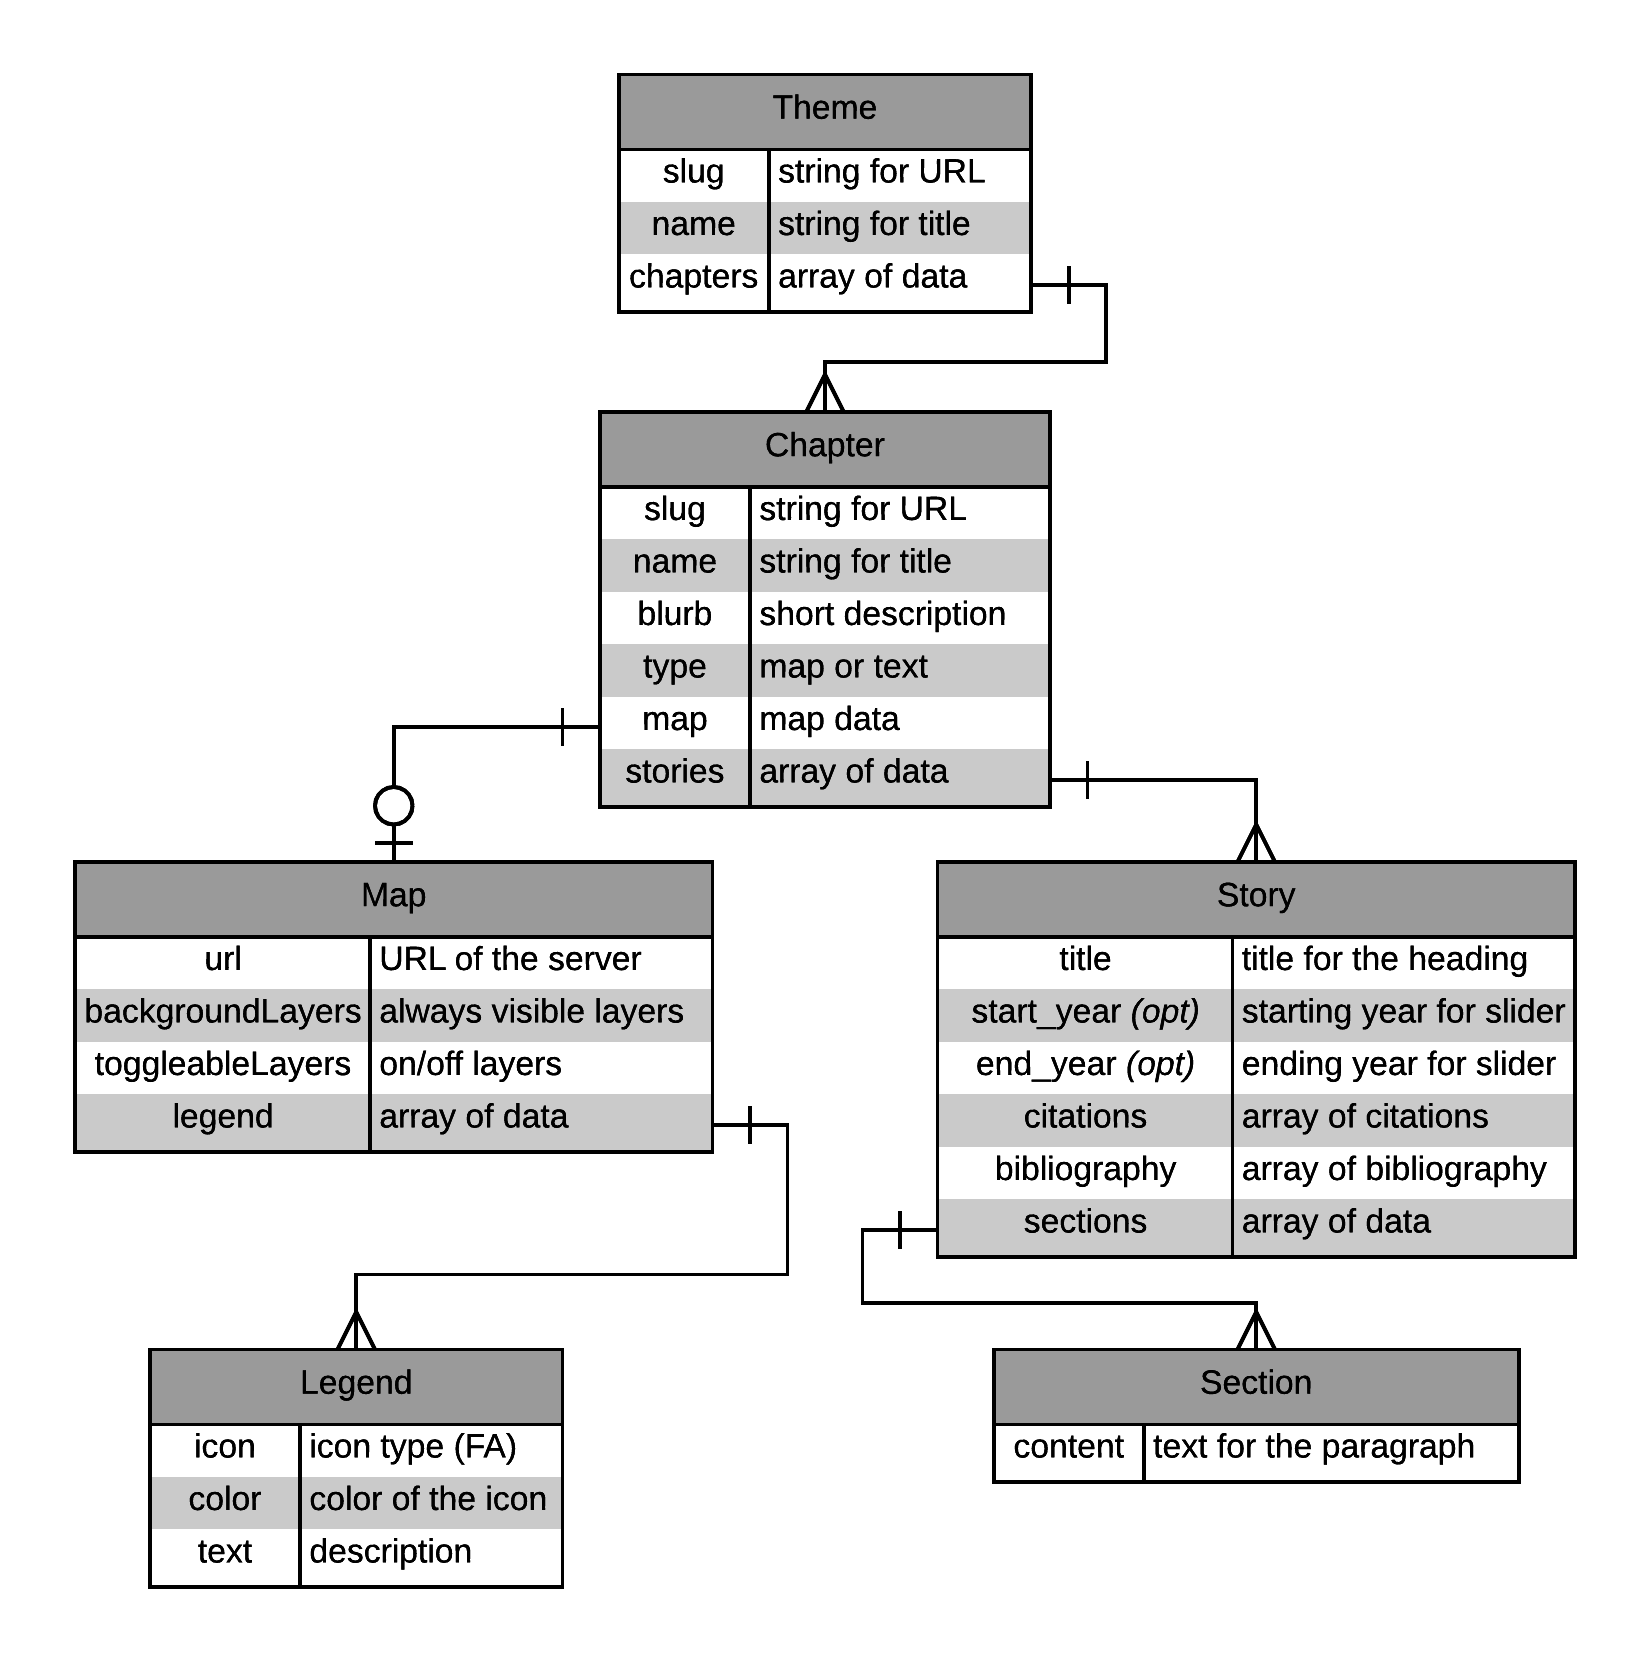
\includegraphics[width=0.45\textwidth]{database_design}
	\caption{AtlasCMS object-oriented database design.}
	\label{fig:database_design}
\end{figure}

\subsection{Slider Creation}
\label{sec:slider_creation}
To increase the interactivity of the atlas, a slider is automatically created for chapters with maps based on the defined toggleable layers for the map. Each toggleable layer is expected to be named with the following format: YYYY$text$, where YYYY is a four-digit year and text can be any text to clarify the layer: e.g. population, ancestry, etc. This ensures that a year can be parsed for the layer, allowing the dynamic creation of the slider on-the-fly. The pseudocode for the parsing of years is in Procedure~\ref{alg:prepare_layers}.

\begin{algorithm}
	\begin{algorithmic}
		\Require $Map$: Map object from database
		\Require $layer$: ArcGISDynamicMaperServiceLayer
		\Ensure $Layers$: Array of years
		
		\State \State $Layers[\ ]\gets [\ ]$
		\ForAll{$Map$.toggleableLayers[\ ] as $layerId$}
			\State $year\gets \Call{parseInt}{layer.$layerInfos$[layerId].$name$}$
			\State \Call{$Layers$.push}{year} 
		\EndFor
	\end{algorithmic}
	\caption{Prepare $Layers$ for slider element}
	\label{alg:prepare_layers}
\end{algorithm}

After the $Layers$ array has been populated with the years, the slider can be created with noUiSlider according to Procedure~\ref{alg:create_slider}.

\begin{algorithm}
	\begin{algorithmic}
		\Require $Map$: Map object from database
		\Require $layer$: ArcGISDynamicMaperServiceLayer
		\Require $Layers$: Array of years
		
		\State \State \Comment{Determine our range of years}
		\State $min\gets Layers[0]$
		\State $max\gets Layers[Layers.$length$ - 1]$
		\State $difference\gets max - min$
		\State $range\gets \{"min``: min, "max``: max\}$
		
		\State \State \Comment{Determine percent of range for each layer}
		\ForAll{$Layers$[\ ] as $year$}
			\State $percent\gets 100 - ((max - year) / difference * 100.0) + "\%``$
			\State $range[percent]\gets year$
		\EndFor
		
		\State \State \Comment{Setup the noUISlider with the ticks}
		\State $start\gets layer.$layerInfos$[Map.$toggleableLayers$[0]].$name$ $
		\State \Call{\$.noUiSlider}{\{\par "start``: $start$,\par "range``: $range$,\par "snap``: true\par \}}
		\State \Call{\$.noUiSlider\_pips}{\{\par "mode``: "values``,\par "density``: 10,\par "values``: $Layers$,\par "stepped``: true\par \}}
	\end{algorithmic}
	\caption{Create slider element}
	\label{alg:create_slider}
\end{algorithm}

Now that the slider element has been created, the onChange function for the slider must be set to change the map when the slider changes, as seen in Procedure~\ref{alg:configure_slider}.

\begin{algorithm}
	\begin{algorithmic}
		\Require $Map$: Map object from database
		\Require $layer$: ArcGISDynamicMaperServiceLayer
		\Require $Layers$: Array of years

		\State \State \Comment{Add the background layers}
		\State $currentLayer[\ ]\gets [\ ]$
		\ForAll{$Map$.backgroundLayers as $backgroundLayer$}
			\State \Call{$currentLayers$.push}{$backgroundLayer$}
		\EndFor
		
		\State \State \Comment{Add in the current toggled layer}
		\State \Call{$currentLayers$.push}{getCurrentLayer()}
		\State \Call{$layer$.setVisibleLayers}{$currentLayers$}
		
		\State \Function{getCurrentLayer}{}
			\State $val\gets \$.val()$
			\ForAll{$Layers$ as $layer$}
				\If{$val == layer$}
					\State \Return $layer$
				\EndIf
			\EndFor
		\EndFunction
	\end{algorithmic}
	\caption{Tie in slider element with Map}
	\label{alg:configure_slider}
\end{algorithm}

\subsection{Map-Narrative Key Points}
\label{sec:map_narrative_key_points}
To increase the interactivity of the atlas, stories can be given starting years and ending years for which they are pertinent to the map. No stories should overlap in year; however, if stories do overlap, the first story in the database will always be selected; therefore, it is recommended that all stories be kept in chronological order in the database, where possible.

On the database side, the toggleable layers are assumed to be connected to specific years. These years are parsed from the ArcGIS Server with the Query command. These years are then used to create the slider at the bottom of the map, as well as check against the starting and ending years of the stories to determine the corresponding story when the year is changed.

Along with Procedure~\ref{alg:configure_slider}, we add to the onChange event for the slider the ability to automatically scroll to the corresponding story, based on year, in the narrative, as shown in Procedure~\ref{alg:map_toggle_slider}.

\begin{algorithm}
	\begin{algorithmic}
		\Require $startYears$: Array of starting years
		\Require $endYears$: Array of ending years
		\Require $oldLayer$: Index of the last layer toggled
		
		\For{$iYear = 0; iYear < startYears.$length$; iYear = iYear + 1$}
			\If{$startYears[iYear]\leq \$(this).$val()$ $}
				\If{$endYears[iYear] > \$(this).$val()$ \&\& iYear\neq oldLayer$}
					\State $oldLayer\gets iYear$
					\State \Comment{animate story DOM to offset}
					\State \Return break
				\EndIf
			\EndIf
		\EndFor
	\end{algorithmic}
	\caption{Scroll to story when slider changes}
	\label{alg:map_toggle_slider}
\end{algorithm}

\section{Results}
Unfortunately, all of the features desired could not be accomplished within the 9 months of work on AtlasCMS. Most notably, the content management portion of the system was put on hold to allow for full completion of the underlying functionality in order to create a fully working website. However, all major components were integrated into the system, as will be demonstrated in the figures to follow.

\subsection{Landing Page}
The landing page is the first page the user encounters when using AtlasCMS. Therefore, the page must clearly present the name of the project, the purpose of the project, and allow navigation into the project. To this end, the landing page uses large divisions between sections and provides a background with an image of the state of North Dakota, giving a consistent feel and logical separation as you scroll through the page.

Figure~\ref{fig:home_top} shows the initial view of the landing page. The user can clearly see the name of the project, presented with a semi-transparent UND green background, and can easily click links to learn about the project, how the project was developed, and the team that developed the project. The user can also click to enter the atlas, or use the top navigation to navigate within the atlas.

\begin{figure}[h!]
	\centering
	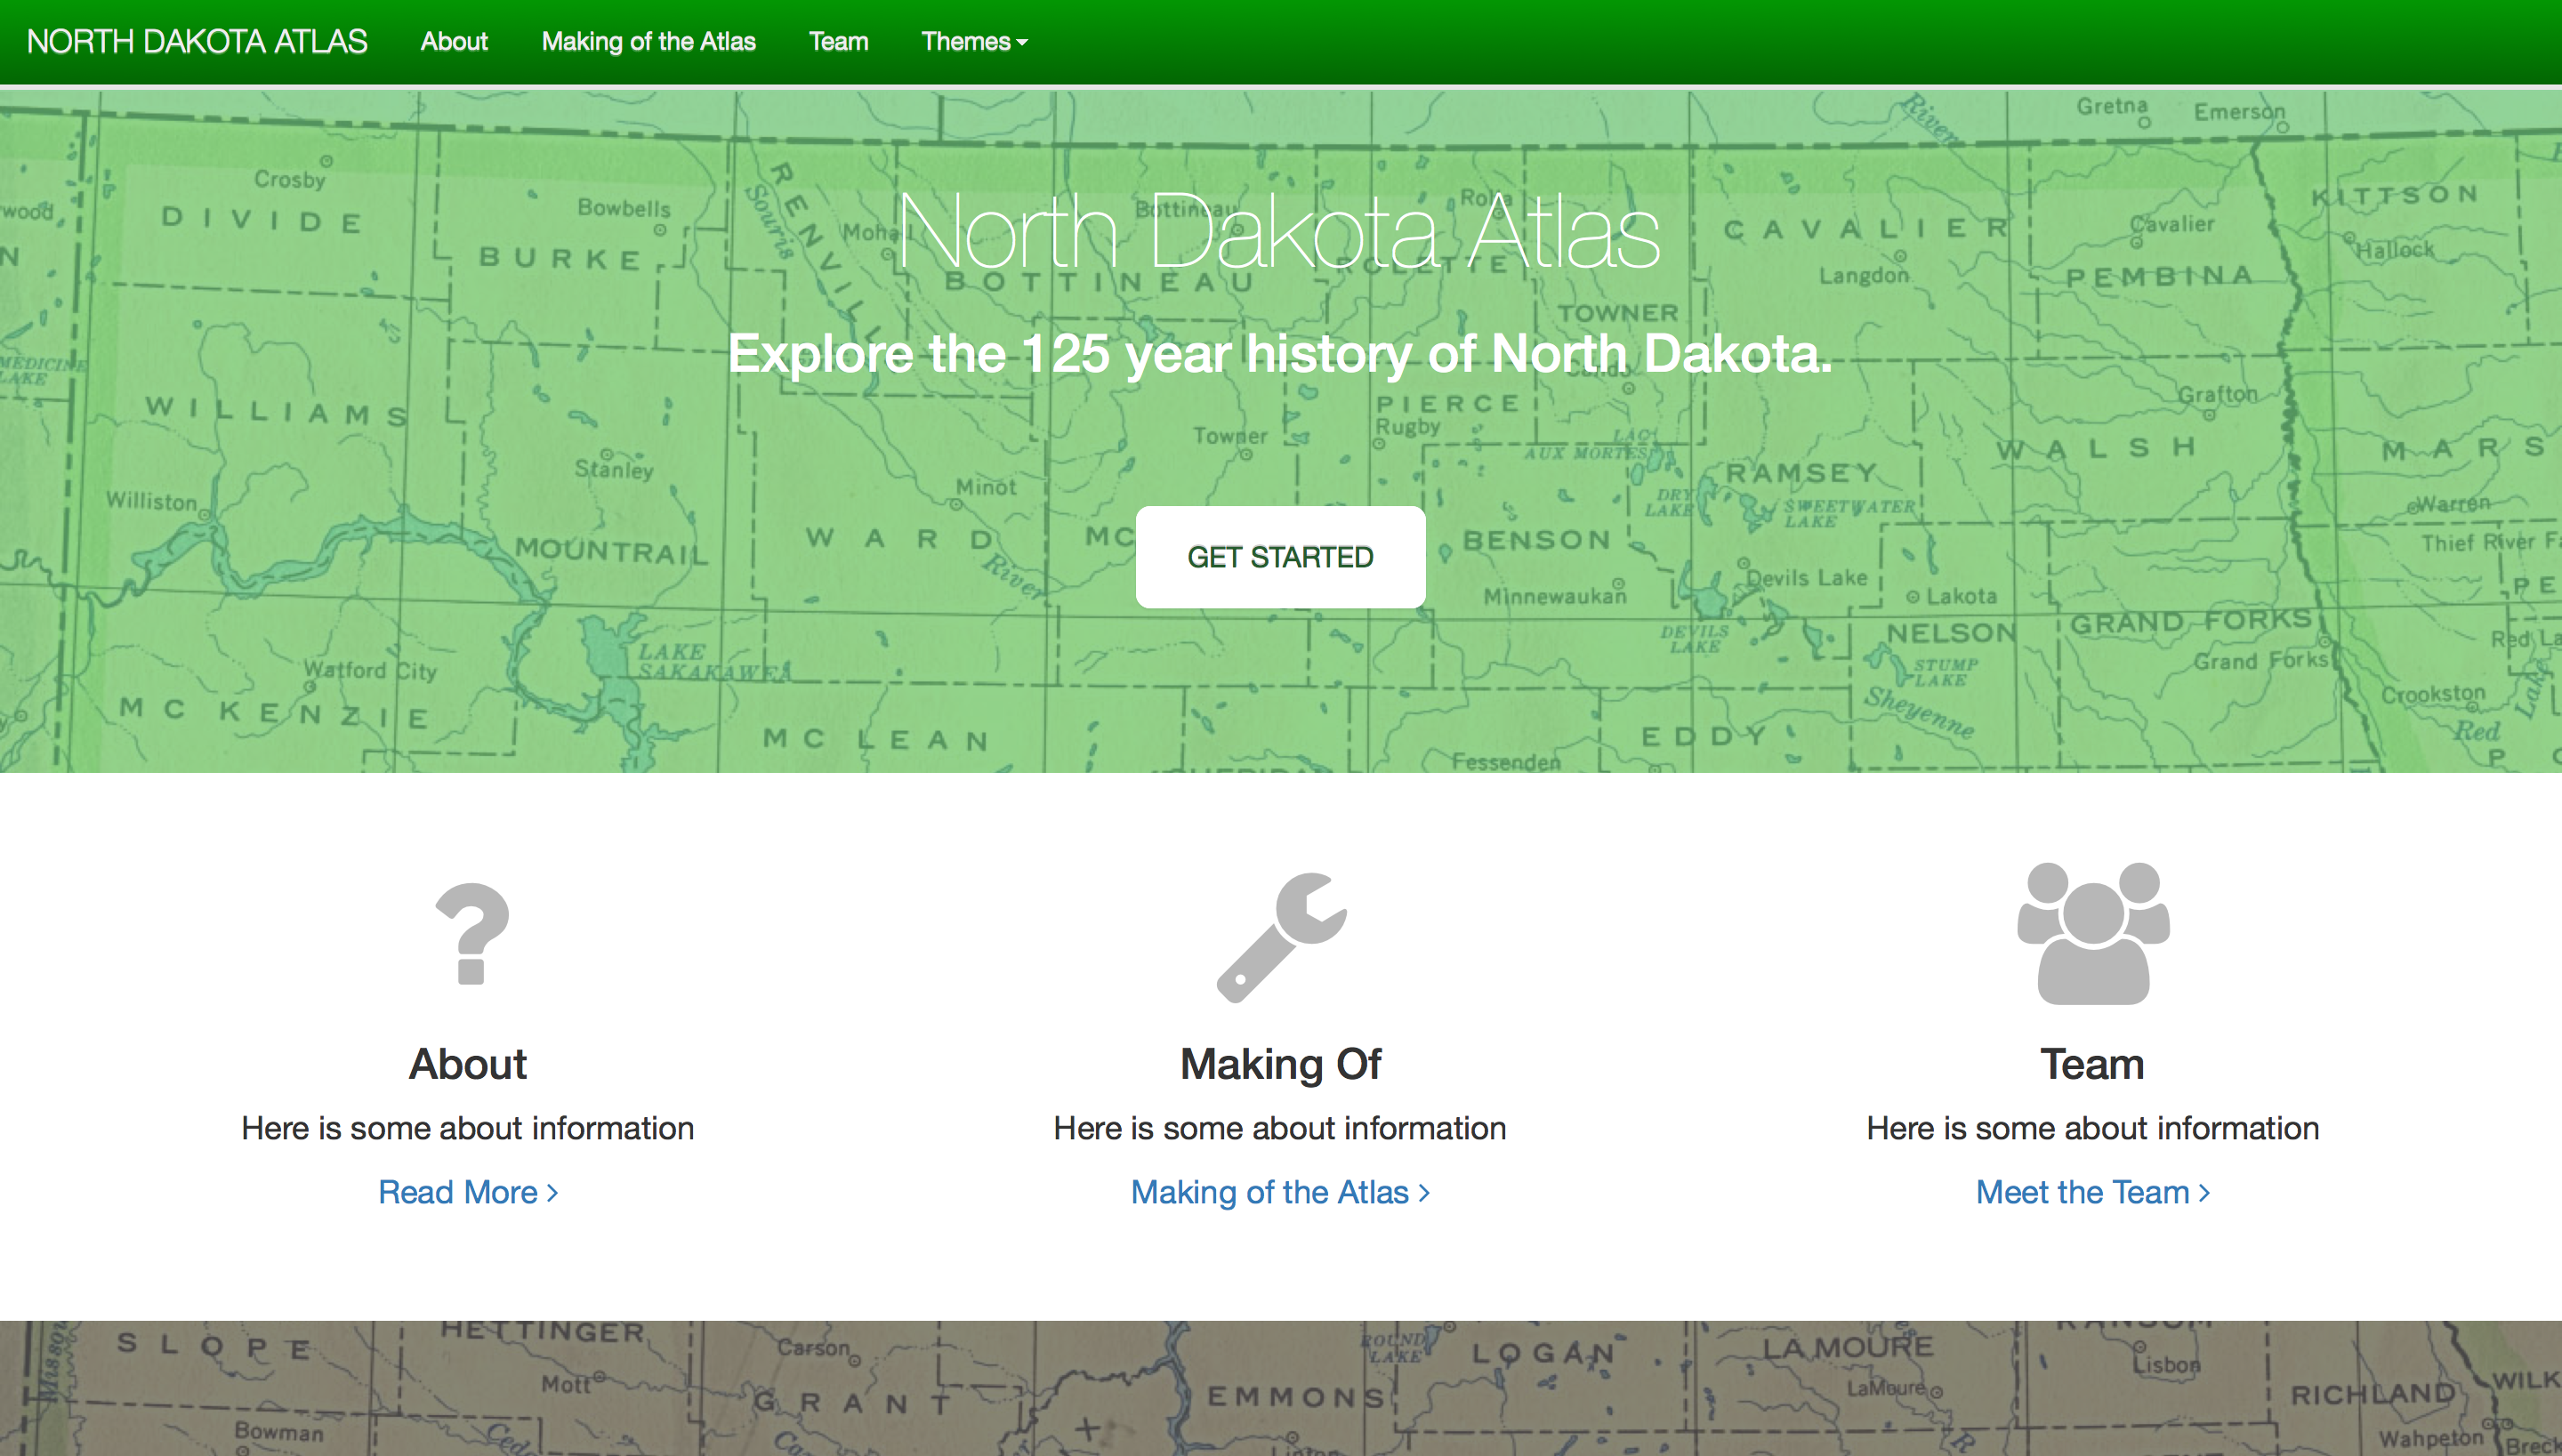
\includegraphics[width=0.45\textwidth]{home_top}
	\caption{AtlasCMS landing page, top.}
	\label{fig:home_top}
\end{figure}

If the user clicks on the About section, they are automatically scrolled to a section that describes the project, as seen in Figure~\ref{fig:home_about}. As can be seen in the figure, the text sections are presented on a solid white background, while the section dividers are transparent black, allowing the North Dakota state image to been seen through. This creates a logical separation and allows for the placement of quotes or other information about the atlas between sections.

\begin{figure}[h!]
	\centering
	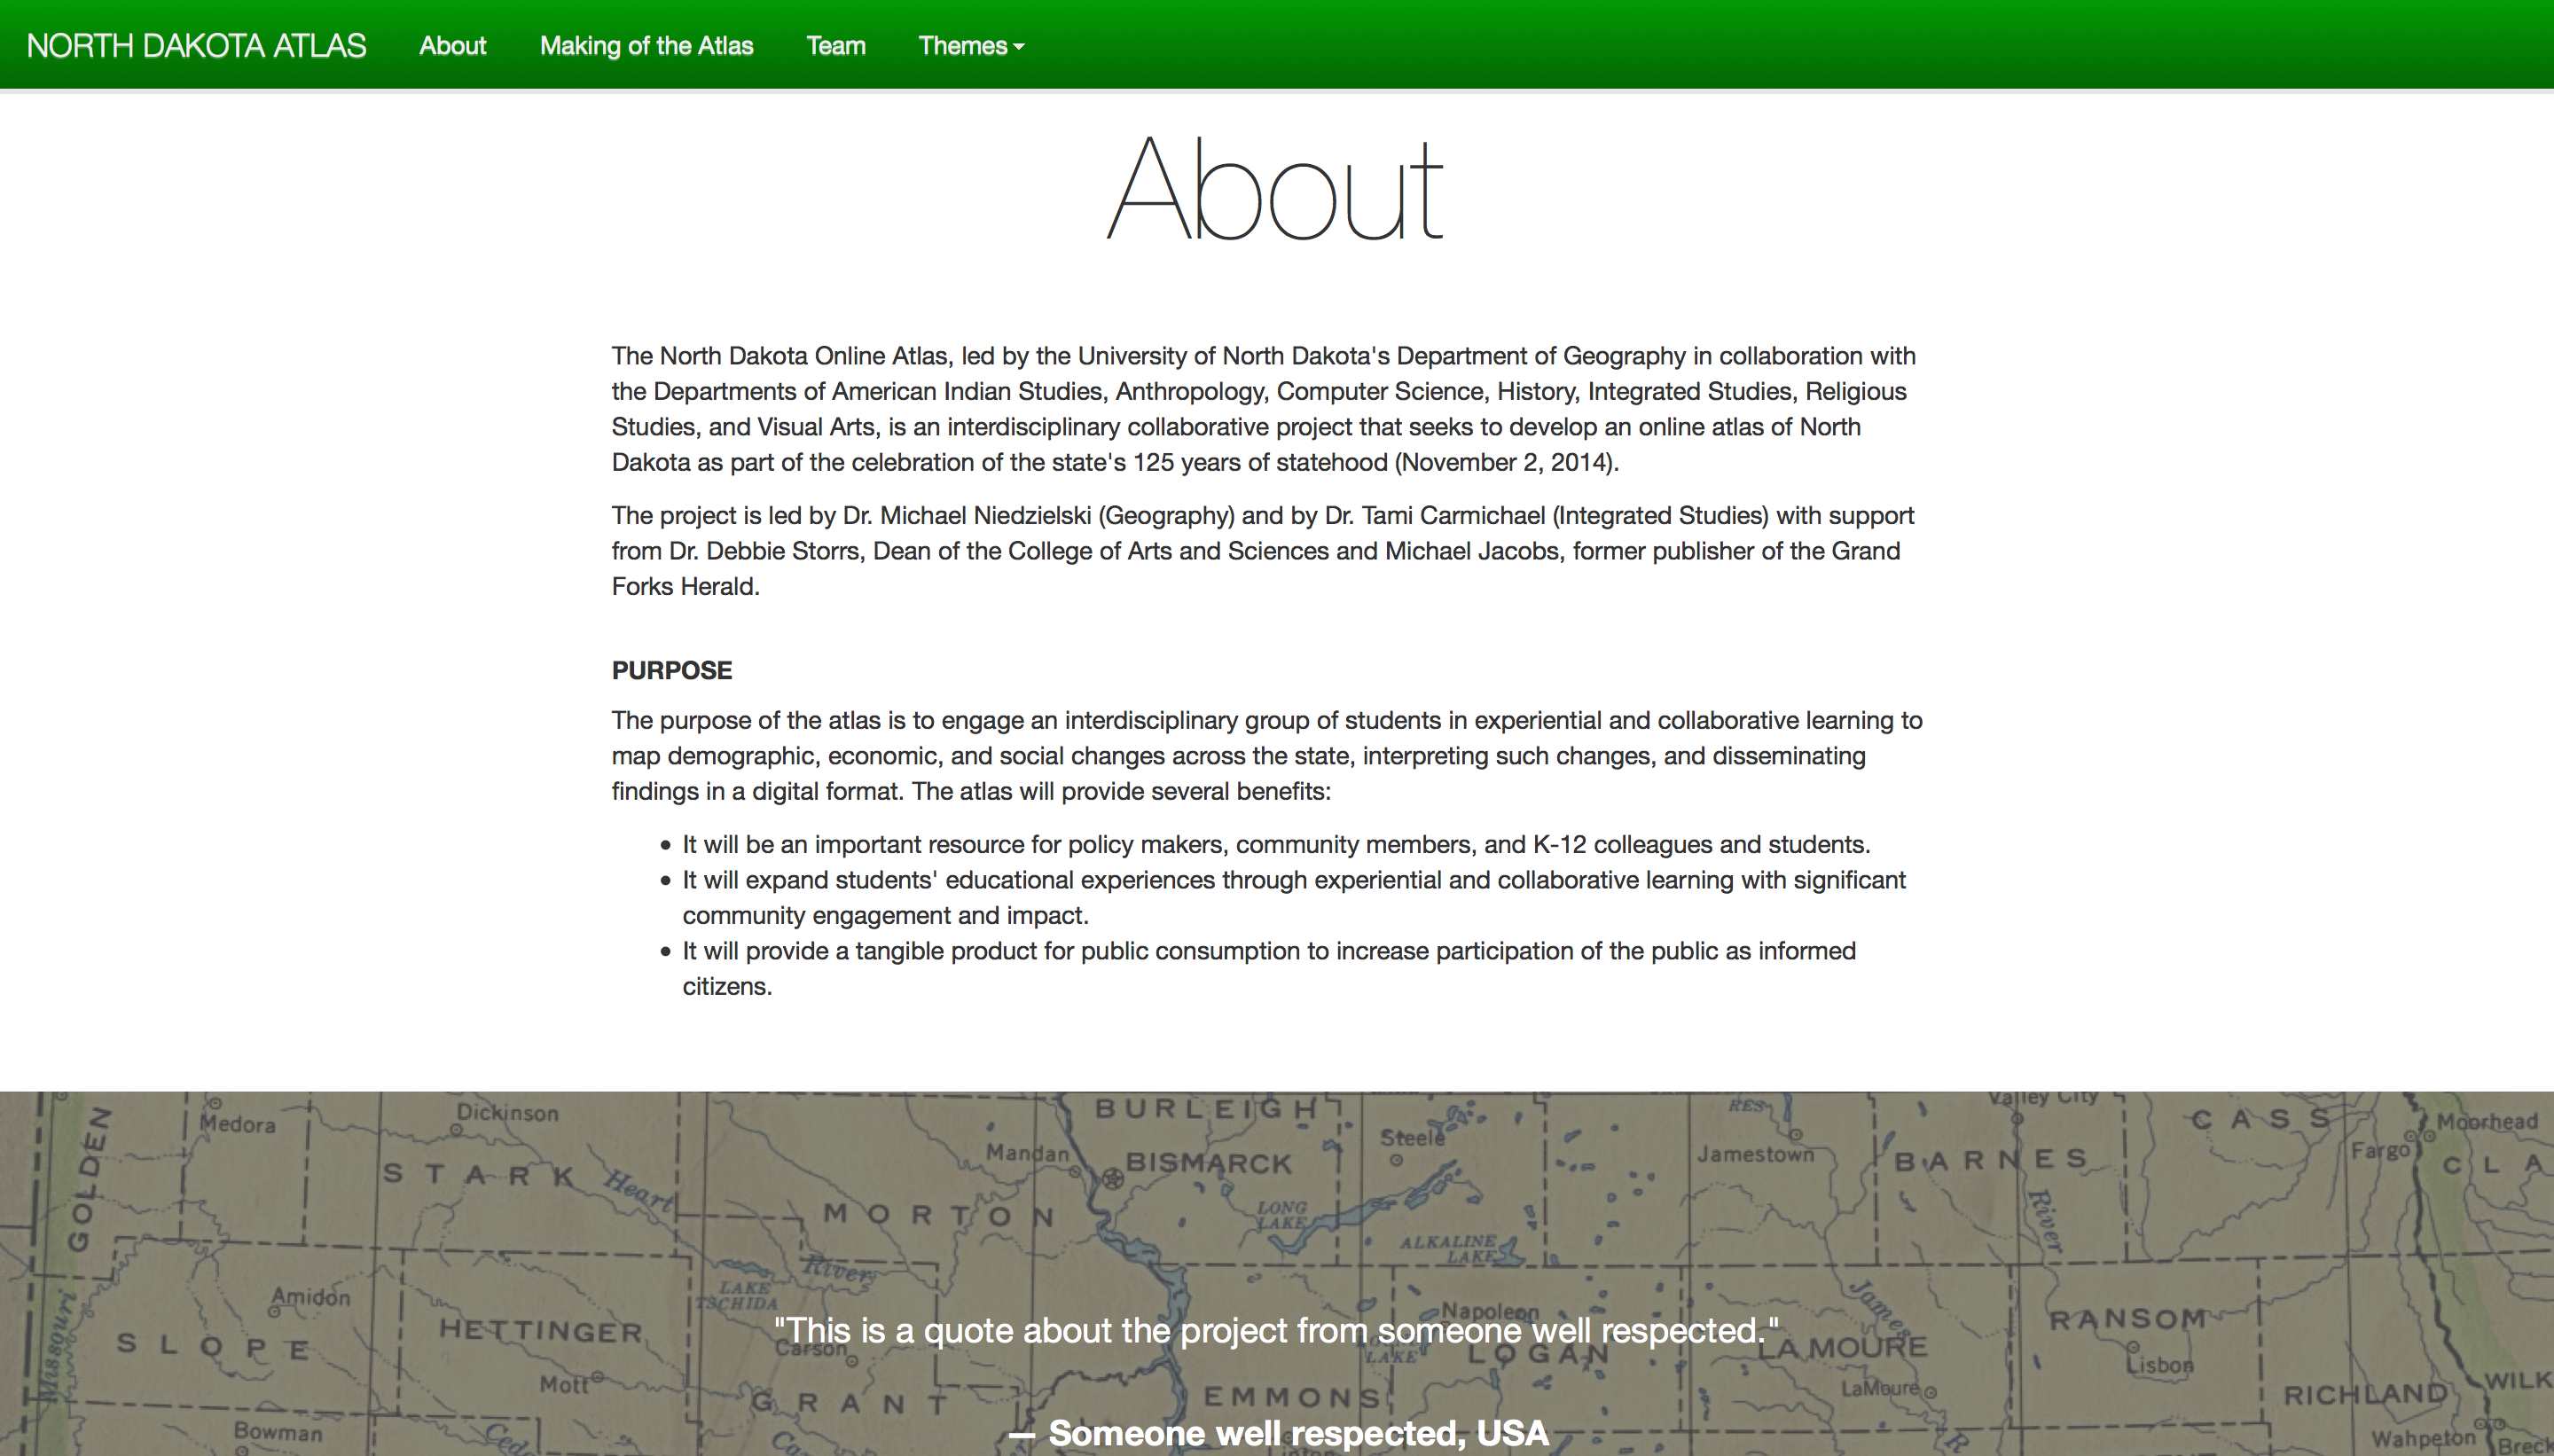
\includegraphics[width=0.45\textwidth]{home_about}
	\caption{AtlasCMS landing page, about.}
	\label{fig:home_about}
\end{figure}

If the user clicks on the Making Of section, they are automatically scrolled to a section that describes the different groups involved int he project, as seen in Figures~\ref{fig:home_making_1} and~\ref{fig:home_making_2}. Just like the About section, the Making Of section uses a solid white background, while the section dividers, not present in the image, are transparent black. As the CMS portion of AtlasCMS is developed, content managers will be able to add and modify sections to the front page, as necessary, with the same basic layout.

\begin{figure}[h!]
	\centering
	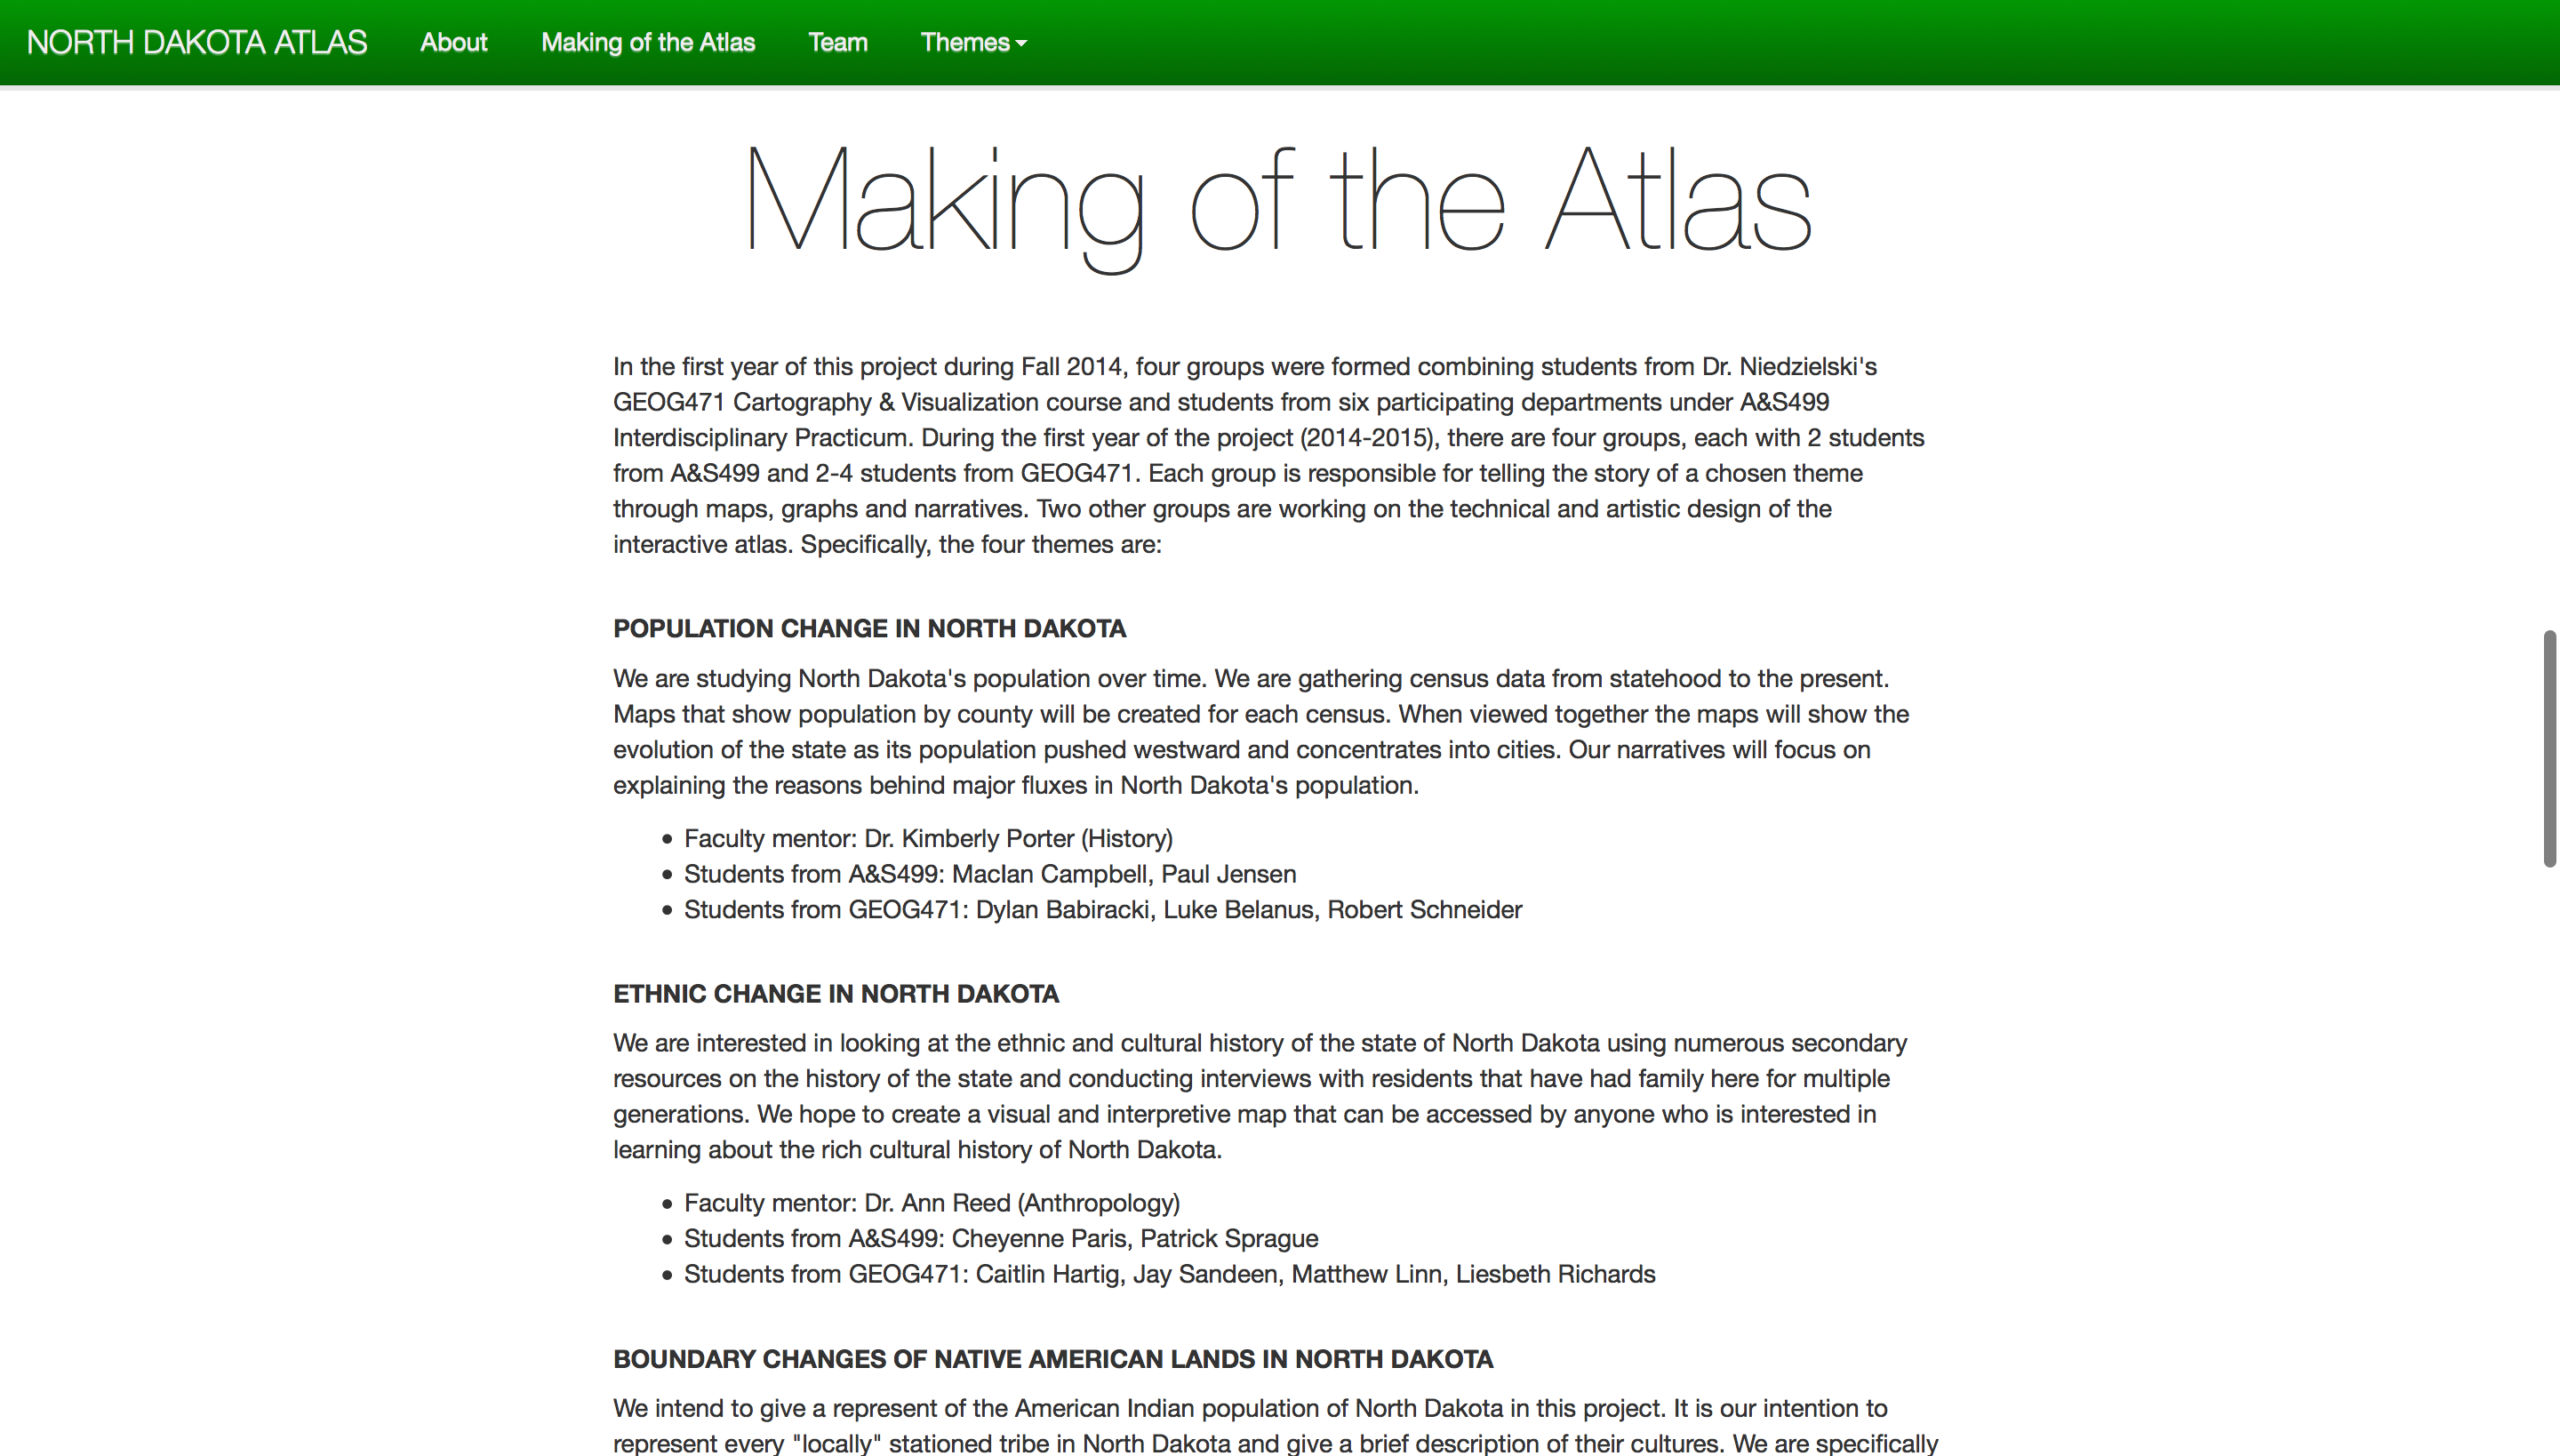
\includegraphics[width=0.45\textwidth]{home_making_1}
	\caption{AtlasCMS landing page, making of.}
	\label{fig:home_making_1}
\end{figure}

\begin{figure}[h!]
	\centering
	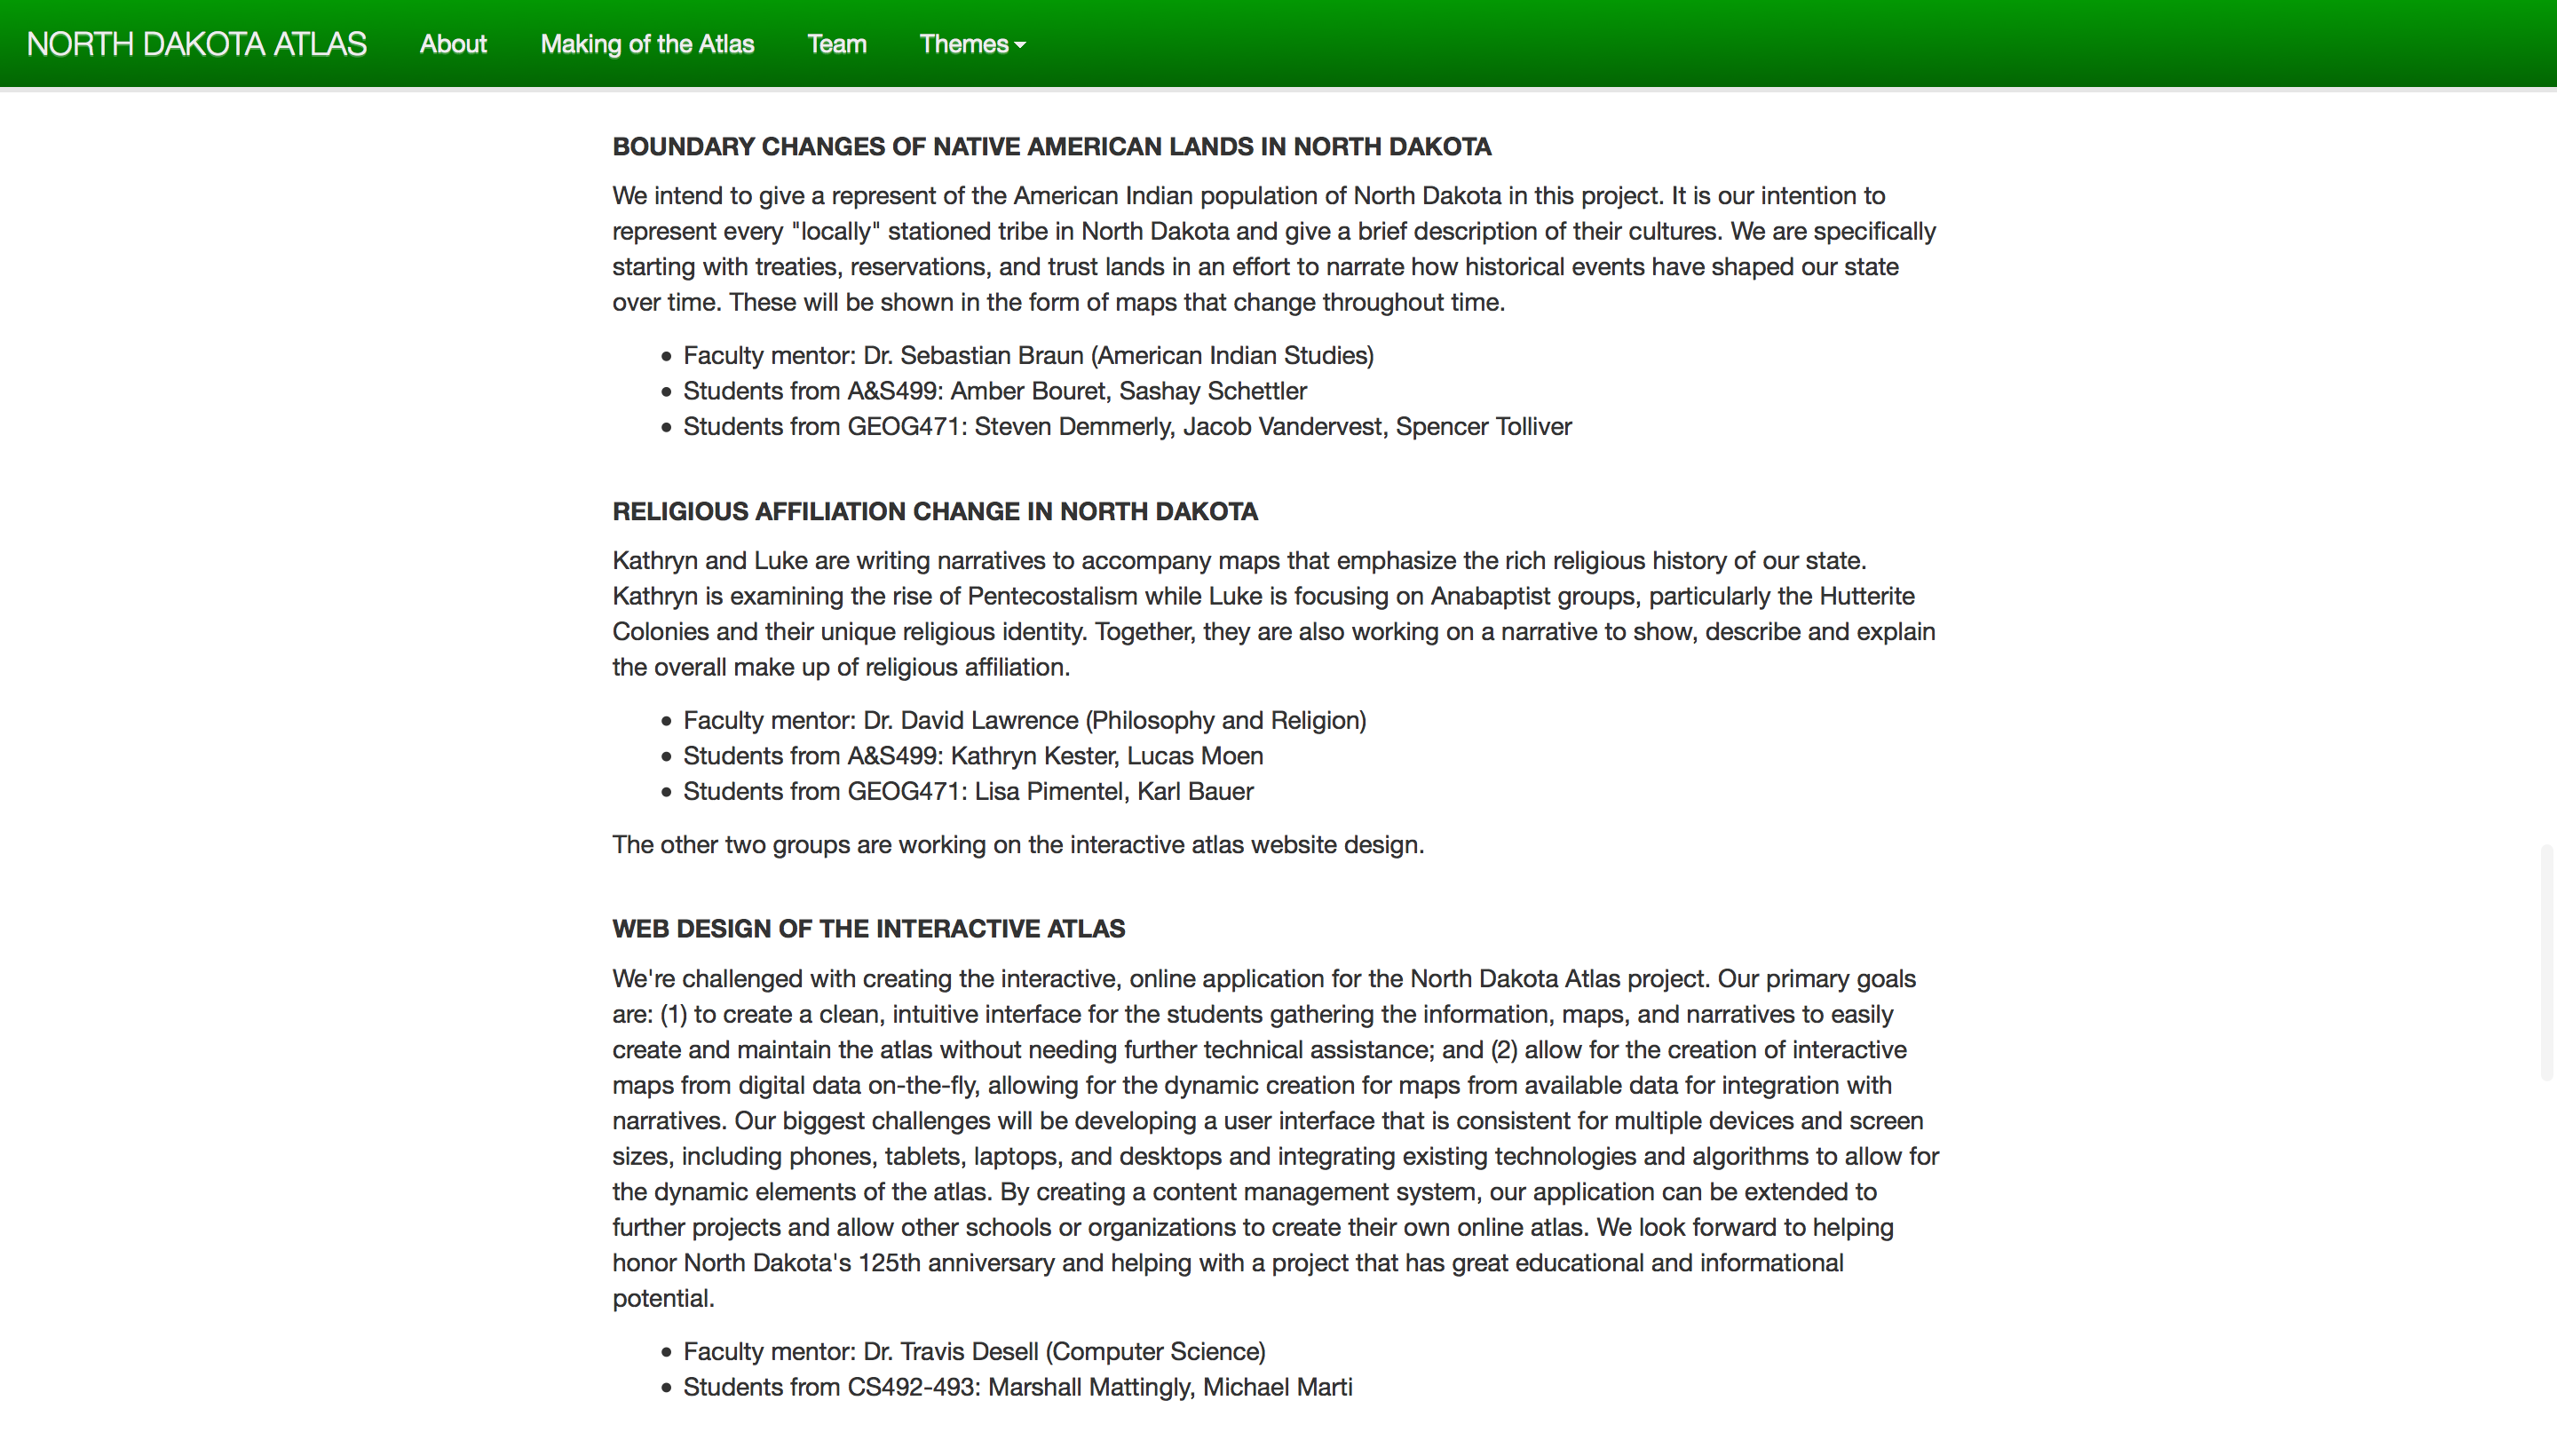
\includegraphics[width=0.45\textwidth]{home_making_2}
	\caption{AtlasCMS landing page, making of.}
	\label{fig:home_making_2}
\end{figure}

If the user clicks on the Team section, they are automatically scrolled to a section with a group photo of the team that worked on the project, as seen in Figure~\ref{fig:home_bottom}. This section shows the footer of the project, which displays the contact information for the project on the left, the University of North Dakota logo in the middle, and convenient links to share the website on multiple social media websites. This footer is also present on narrative pages, placed at the end of the narrative, so that the map can fill the viewport, instead of the bottom of the screen.

\begin{figure}[h!]
	\centering
	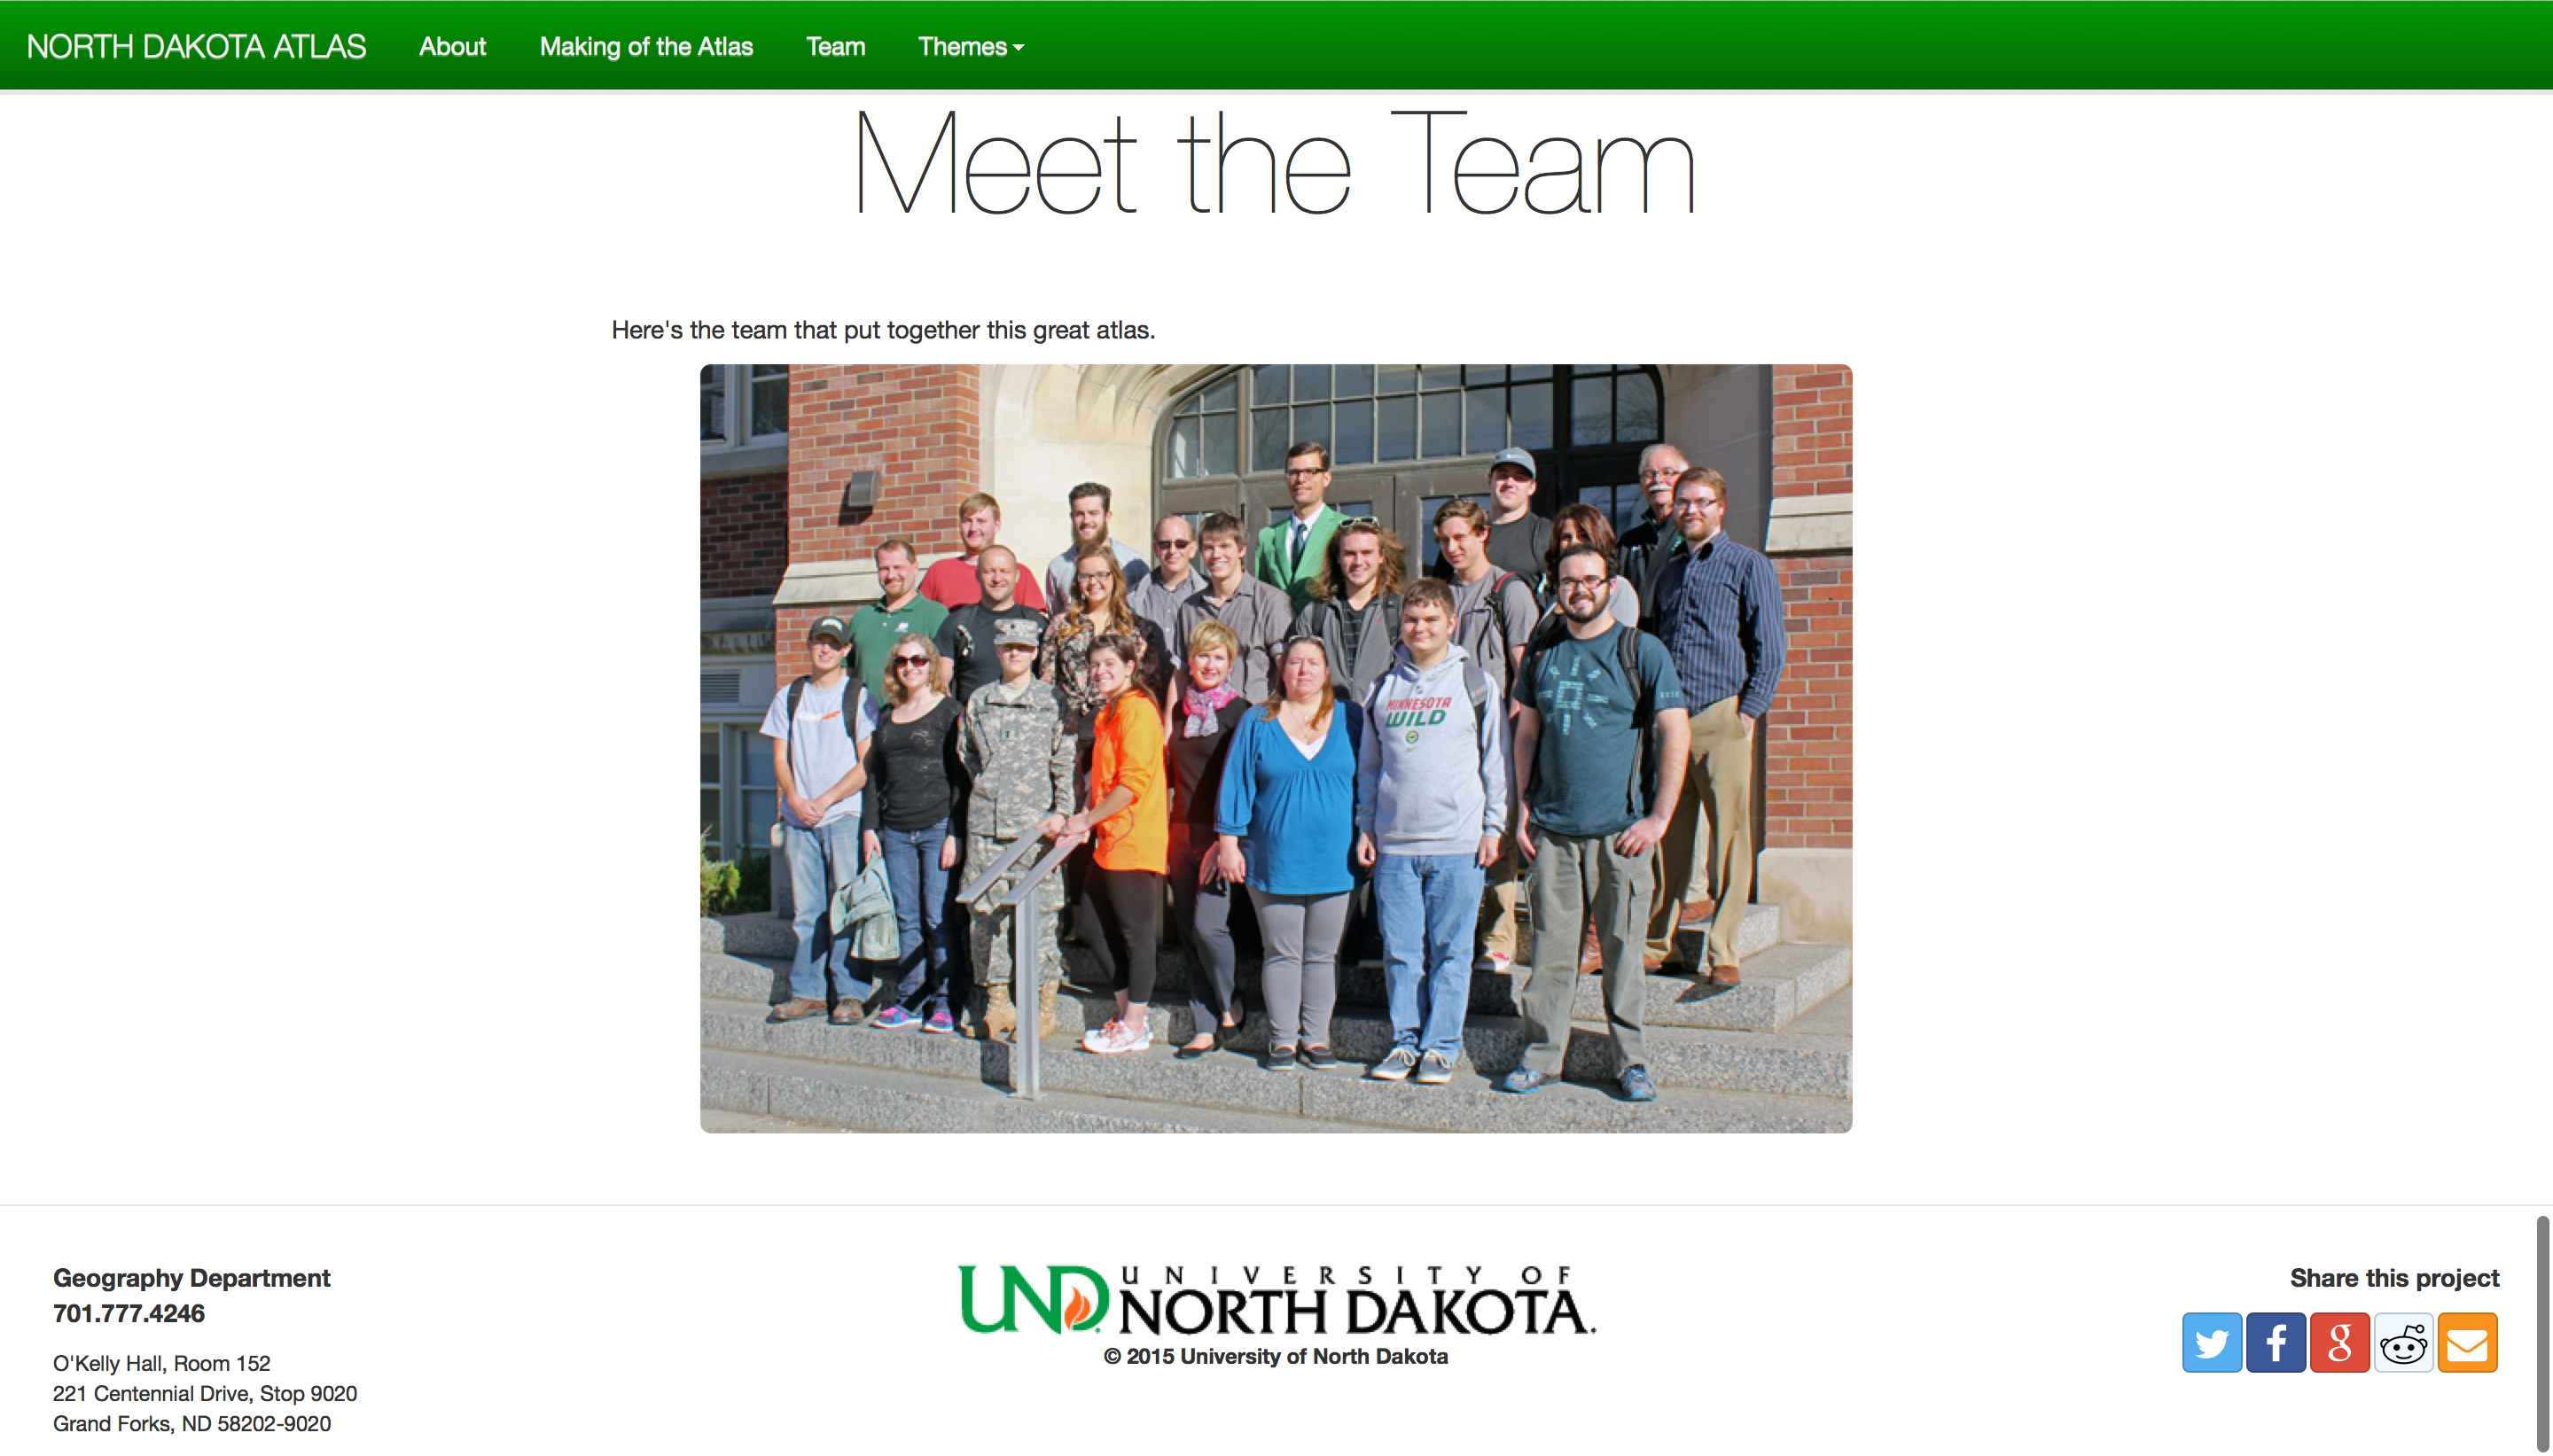
\includegraphics[width=0.45\textwidth]{home_bottom}
	\caption{AtlasCMS landing page, footer.}
	\label{fig:home_bottom}
\end{figure}

As the user shrinks the viewport, the footer automatically re-orders to have the contact information, followed by the sharing links, then ending with a compact version of the UND logo, as seen in Figure~\ref{fig:home_bottom_small}. This shows how AltasCMS has the potential to easily scale to multiple viewports with minimal code changes.

\begin{figure}[h!]
	\centering
	
\includegraphics[width=0.45\textwidth,height=3in,keepaspectratio]{home_bottom_small}
	\caption{AtlasCMS landing page, footer, condensed.}
	\label{fig:home_bottom_small}
\end{figure}

\subsection{History of the State}
This History of the State theme deals with the gross population of North Dakota through time. The map begins in 1890, the founding years of the state, and continues through present time. Figure~\ref{fig:making} shows the initial view when entering the chapter, showing the population as a dot-density map with the slider set to 1890. The main things to notice on the page is the slider, at the bottom of the map, that allows the user to changes years; the narrative on the right side of the page, showing the current narrative for the map; and the map centered on the left-side of the page showing the actual dog-density map, with a legend hovering on the bottom right, scale on the bottom left, and zoom-in/-out on the top-left.

\begin{figure}[h!]
	\centering
	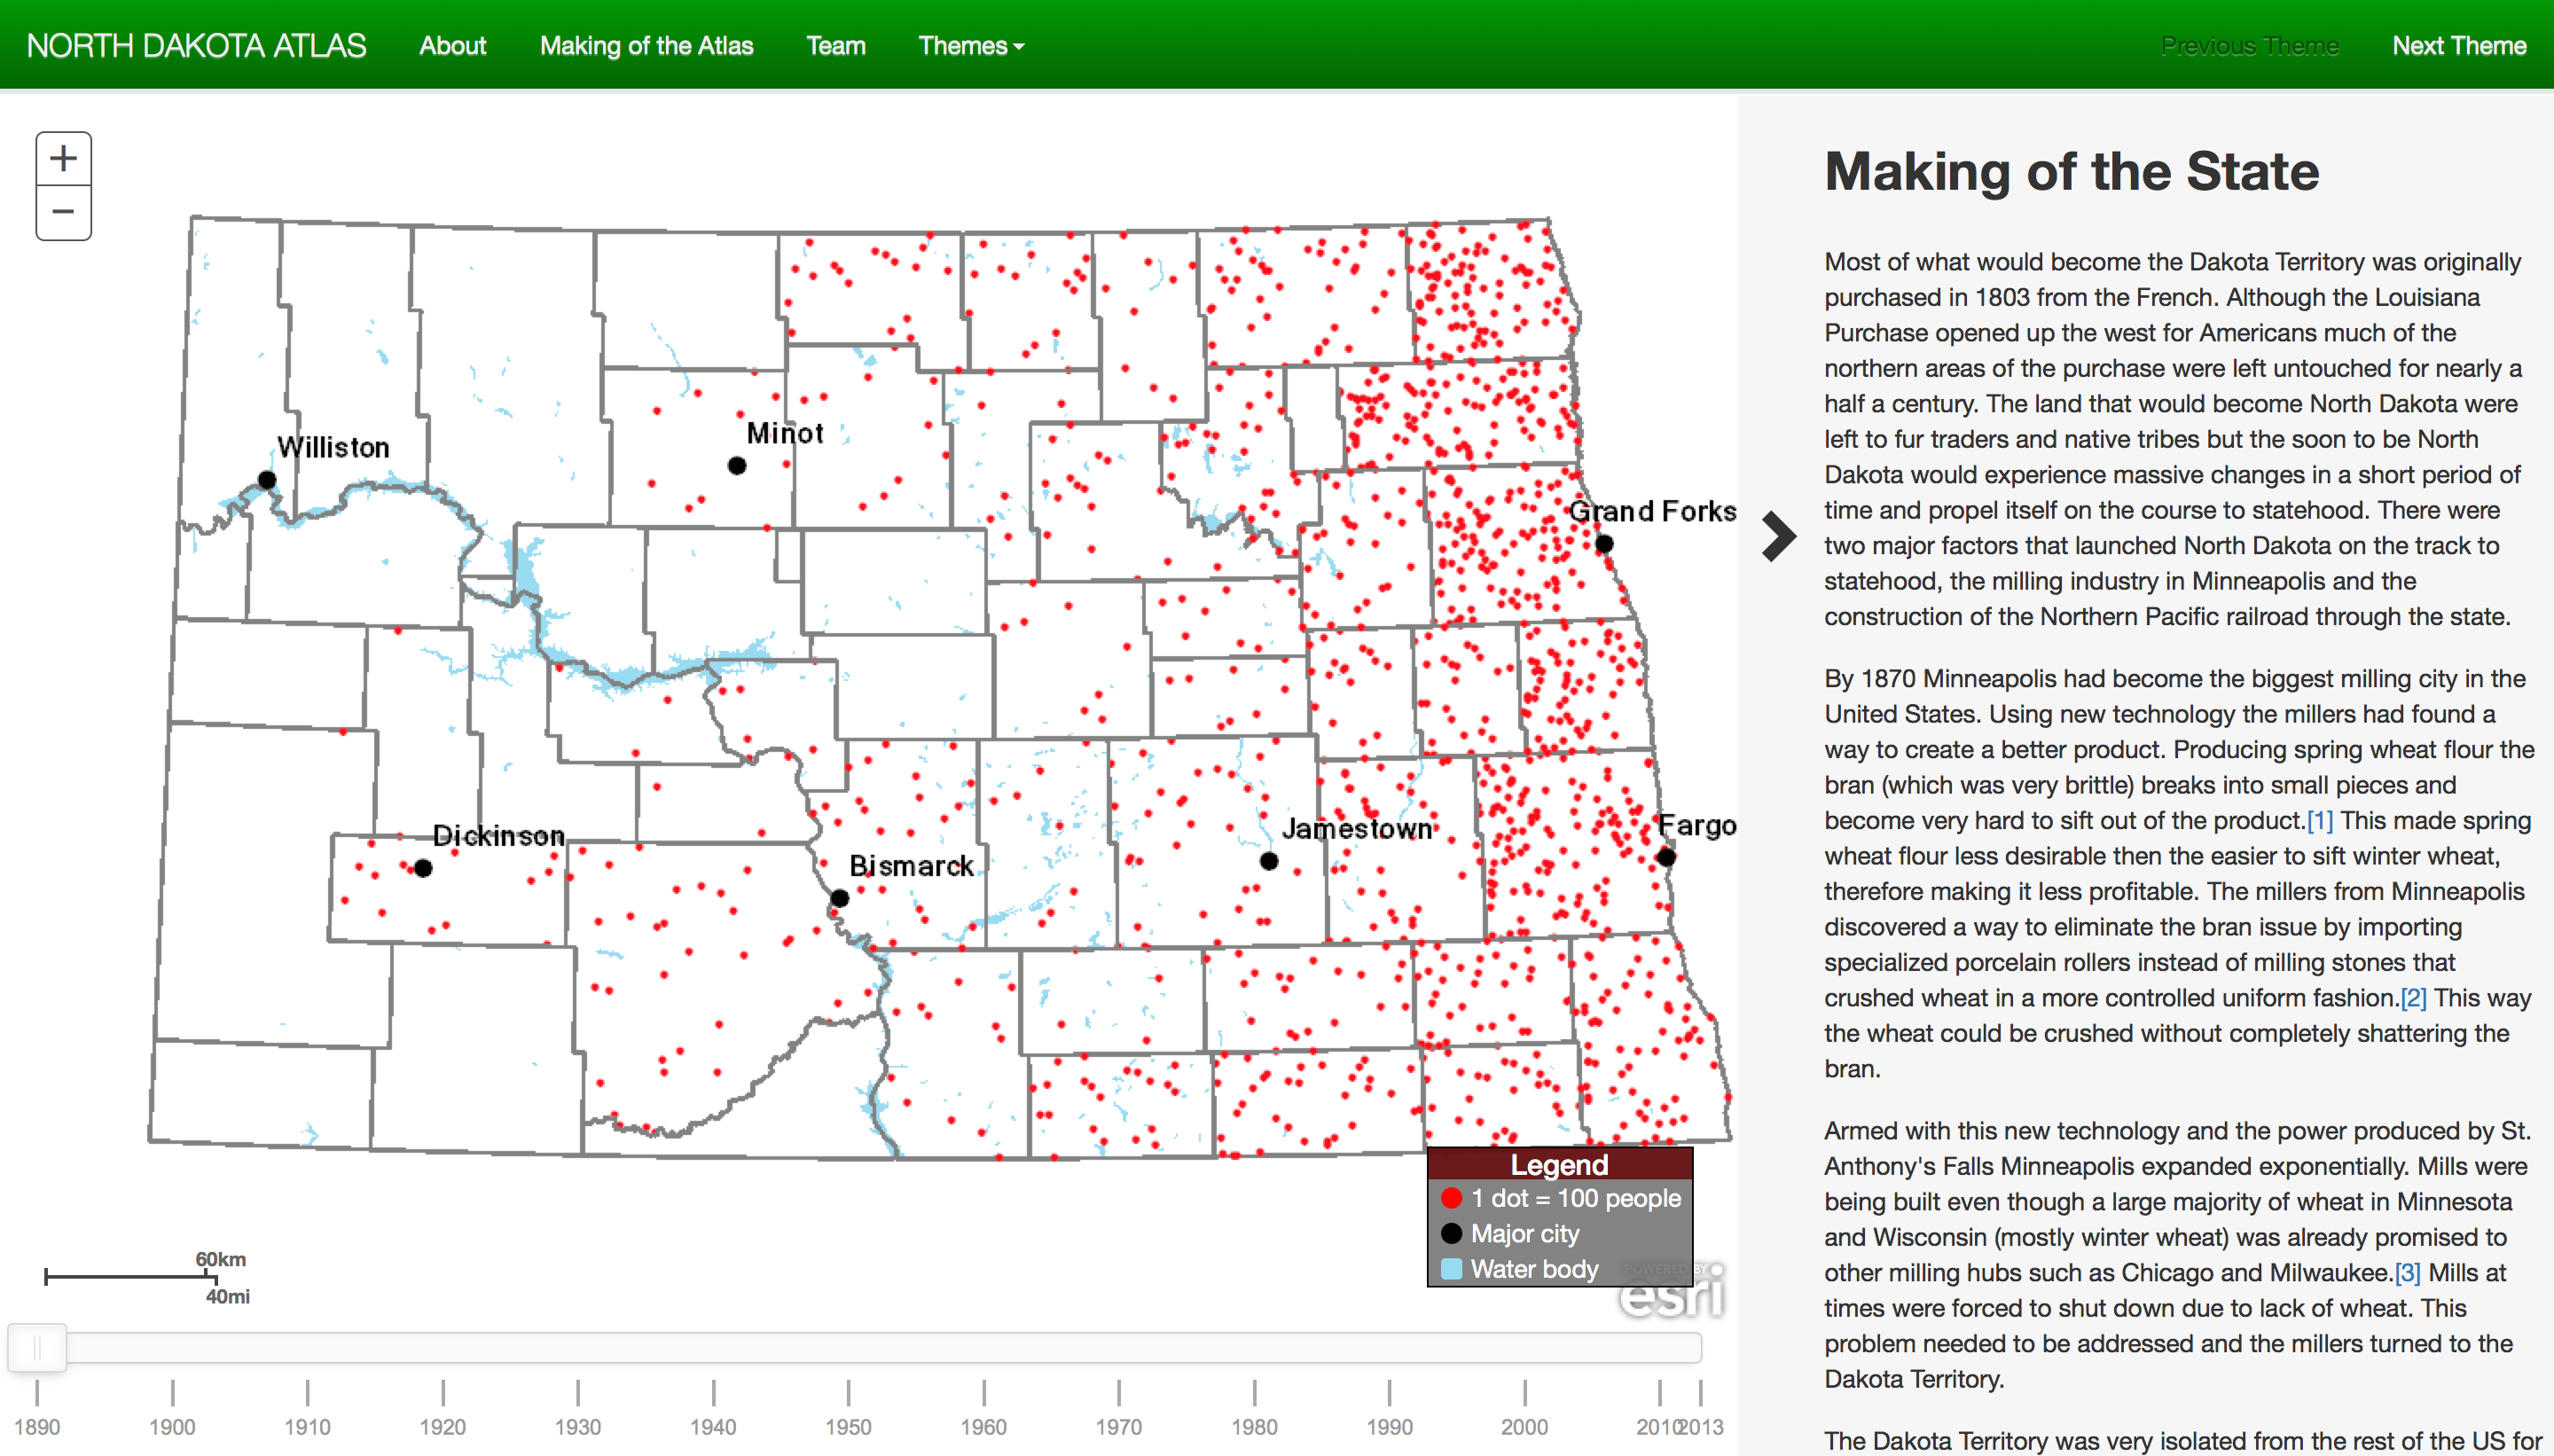
\includegraphics[width=0.45\textwidth]{making}
	\caption{Example map with single-color data.}
	\label{fig:making}
\end{figure}

Given the chronological nature of the map and narrative, this map lends itself well to automatically scrolling the narrative when the slider is changed. As shown in Figure~\ref{fig:making_jump}, when the slider is changed to the year 1960, the narrative automatically scrolled to the Energy Boom narrative, which is centered around the late 1960s to early 1980s. The procedures for handling this are covered in Subsection~\ref{sec:map_narrative_key_points}.

\begin{figure}[h!]
	\centering
	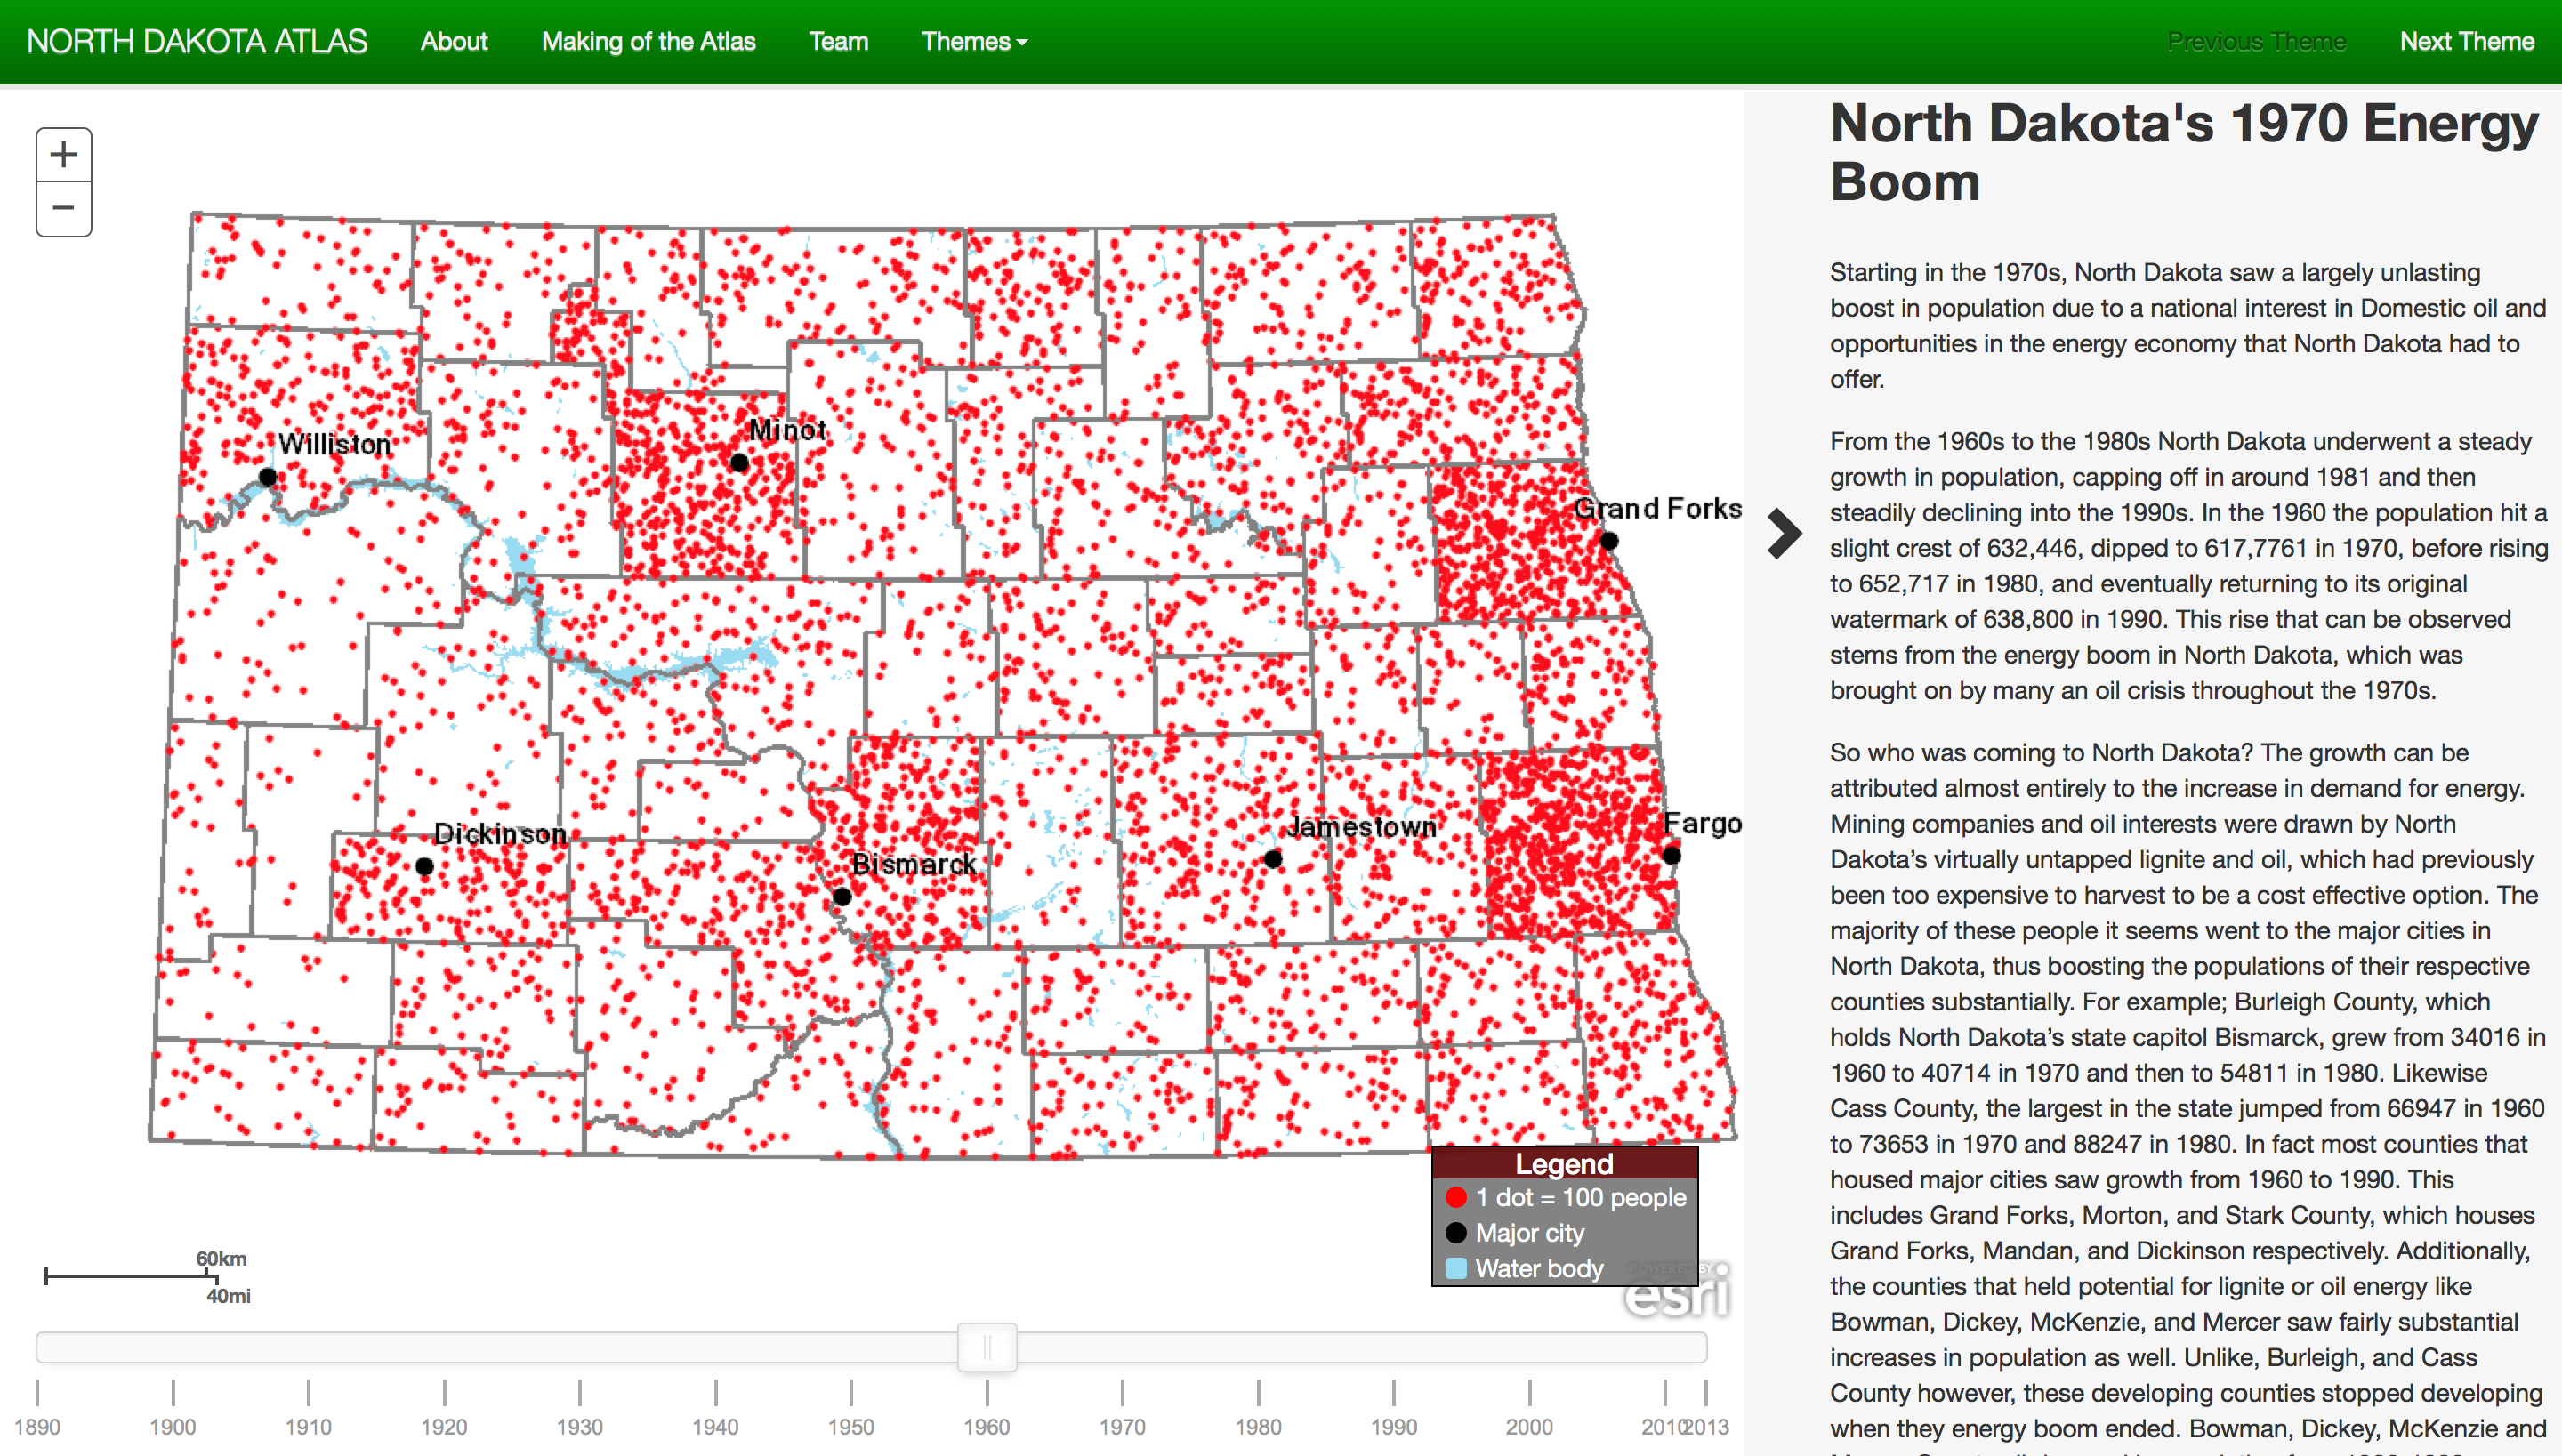
\includegraphics[width=0.45\textwidth]{making_jump}
	\caption{Example of automatic narrative scrolling.}
	\label{fig:making_map}
\end{figure}

\subsection{Anthropology of the State}
The Anthropology of the State deals with the gross populations of three immigrant groups to North Dakota: Germans, Norwegians, and Russians. Just like the History of the State, the map begins in 1890 and continues through present time. Figure~\ref{fig:ancestry} shows the population of the three groups as a dot-density map. The important difference between this map and the History of the State map is the multiple colors and corresponding additions to the legend in the bottom right.

\begin{figure}[h!]
	\centering
	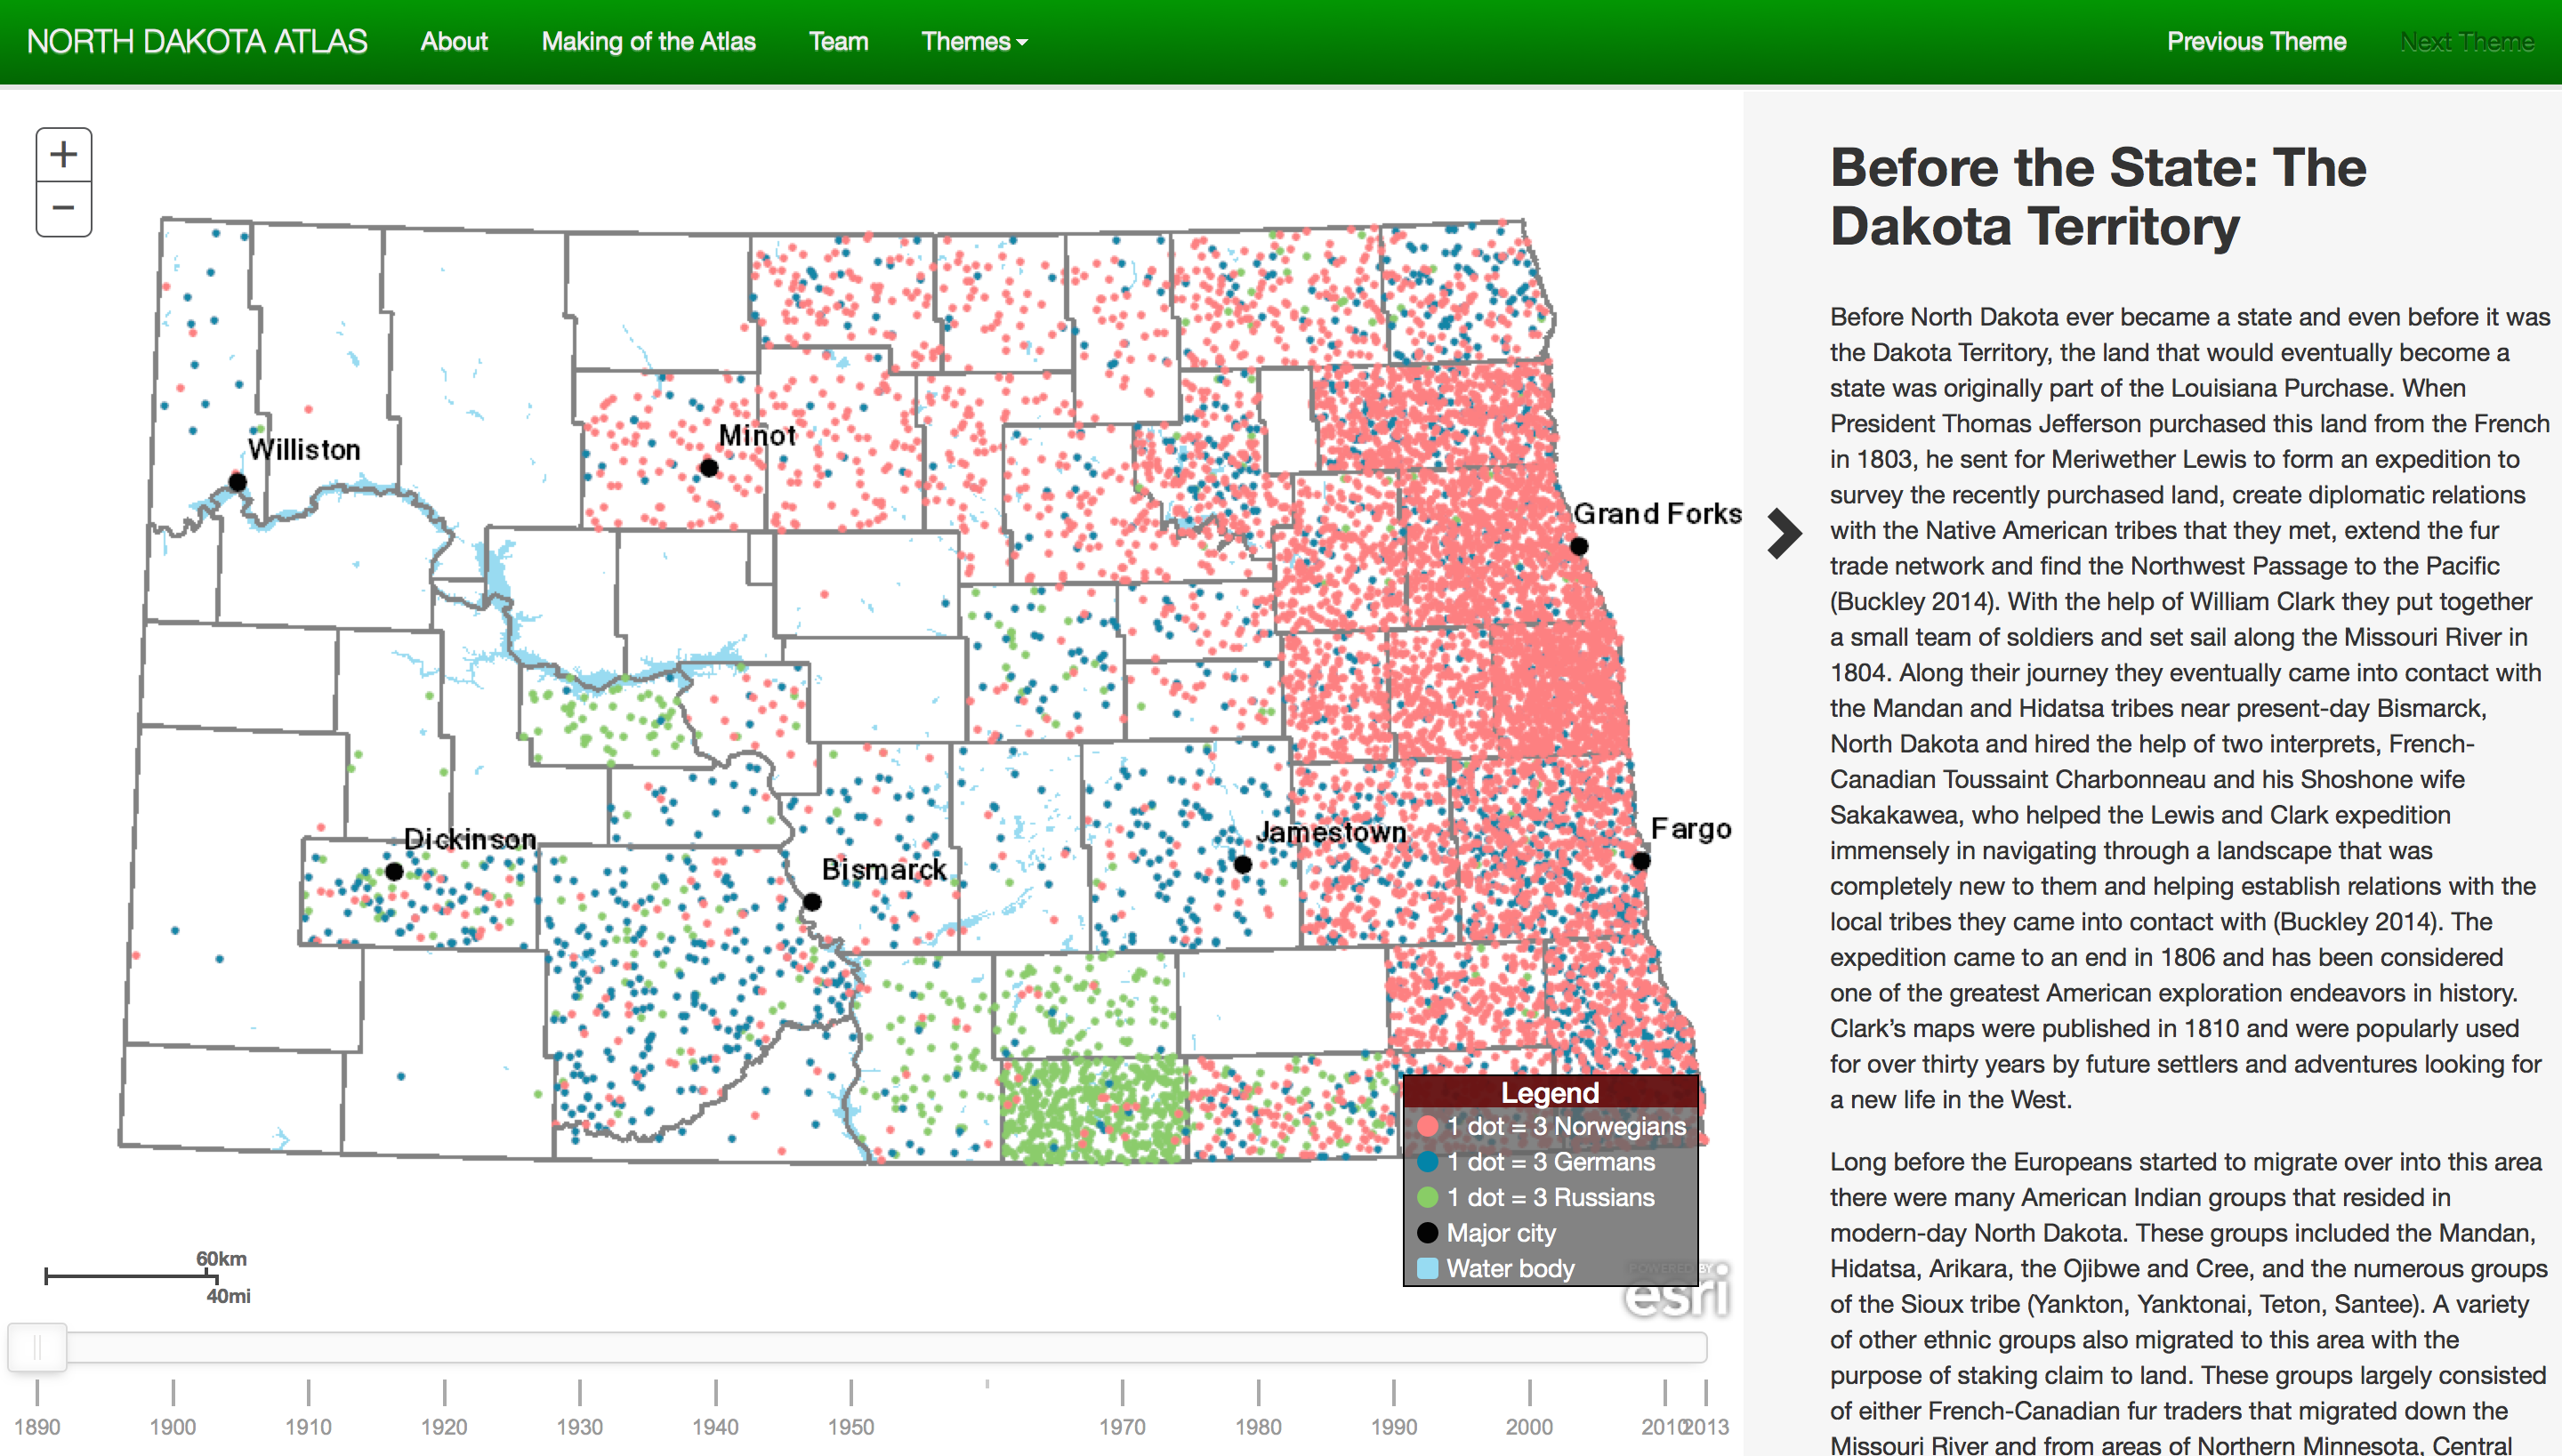
\includegraphics[width=0.45\textwidth]{ancestry}
	\caption{Example map with multiple-color data.}
	\label{fig:ancestry}
\end{figure}

Unlike the History of the State, the anthropology narrative is presented by group, instead of chronologically. Since a single year can reference a different part of the narrative, depending on the ethnic group one is interested in, it is impossible to automatically scroll to a corresponding part of the narrative, as shown in Figure~\ref{fig:ancestry_jump}. One consideration for the future will be to sort all narratives chronologically to allow for automatic narrative scrolling on any page.

\begin{figure}[h!]
	\centering
	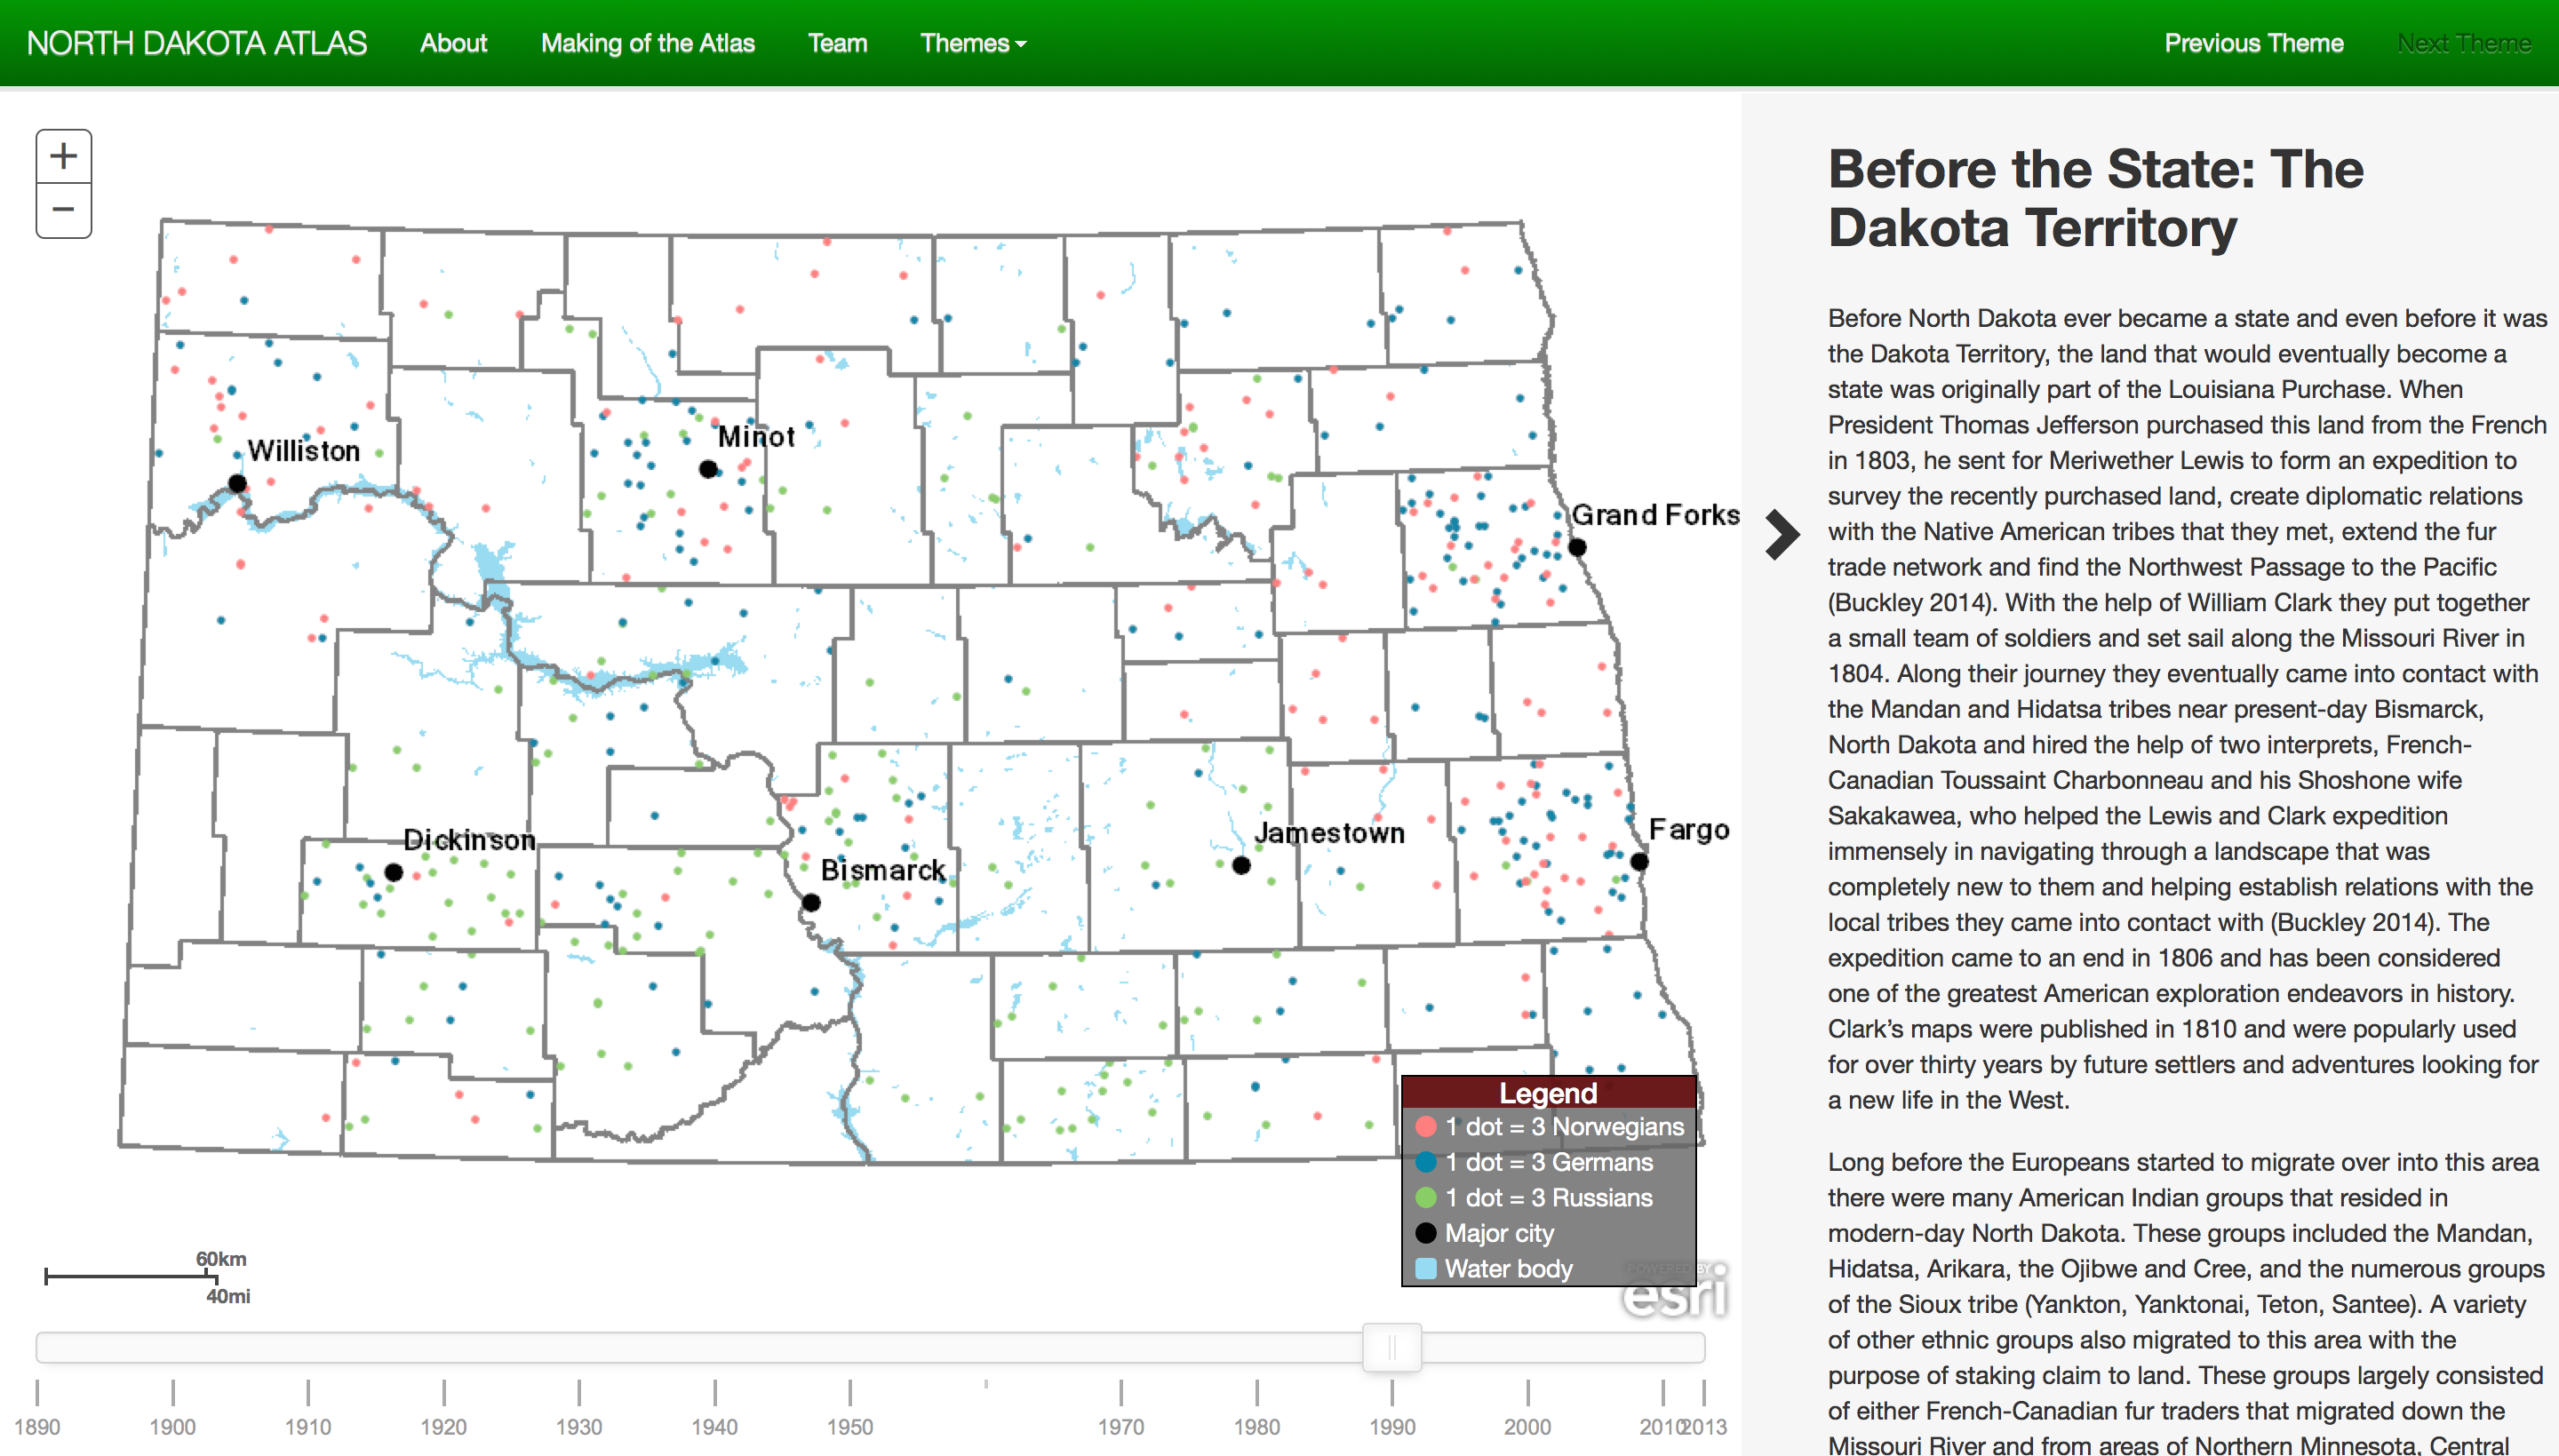
\includegraphics[width=0.45\textwidth]{ancestry_jump}
	\caption{Example of non-automatic narrative scrolling.}
	\label{fig:ancestry_jump}
\end{figure}

To view more of the map, the user is able to hide the narrative by pressing the right-facing chevron to the left of the narrative, as shown in Figure~\ref{fig:ancestry_no_narrative}. The important thing to note when hiding the narrative is the map and scroll bar resize to fill the emptied screen real estate, while the legend follows the right edge. To again show the narrative, the user can click the left-facing chevron. This automatic resizing of the map again shows that AtlasCMS can be fitted to multiple viewports with minimal coding.

\begin{figure}[h!]
	\centering
	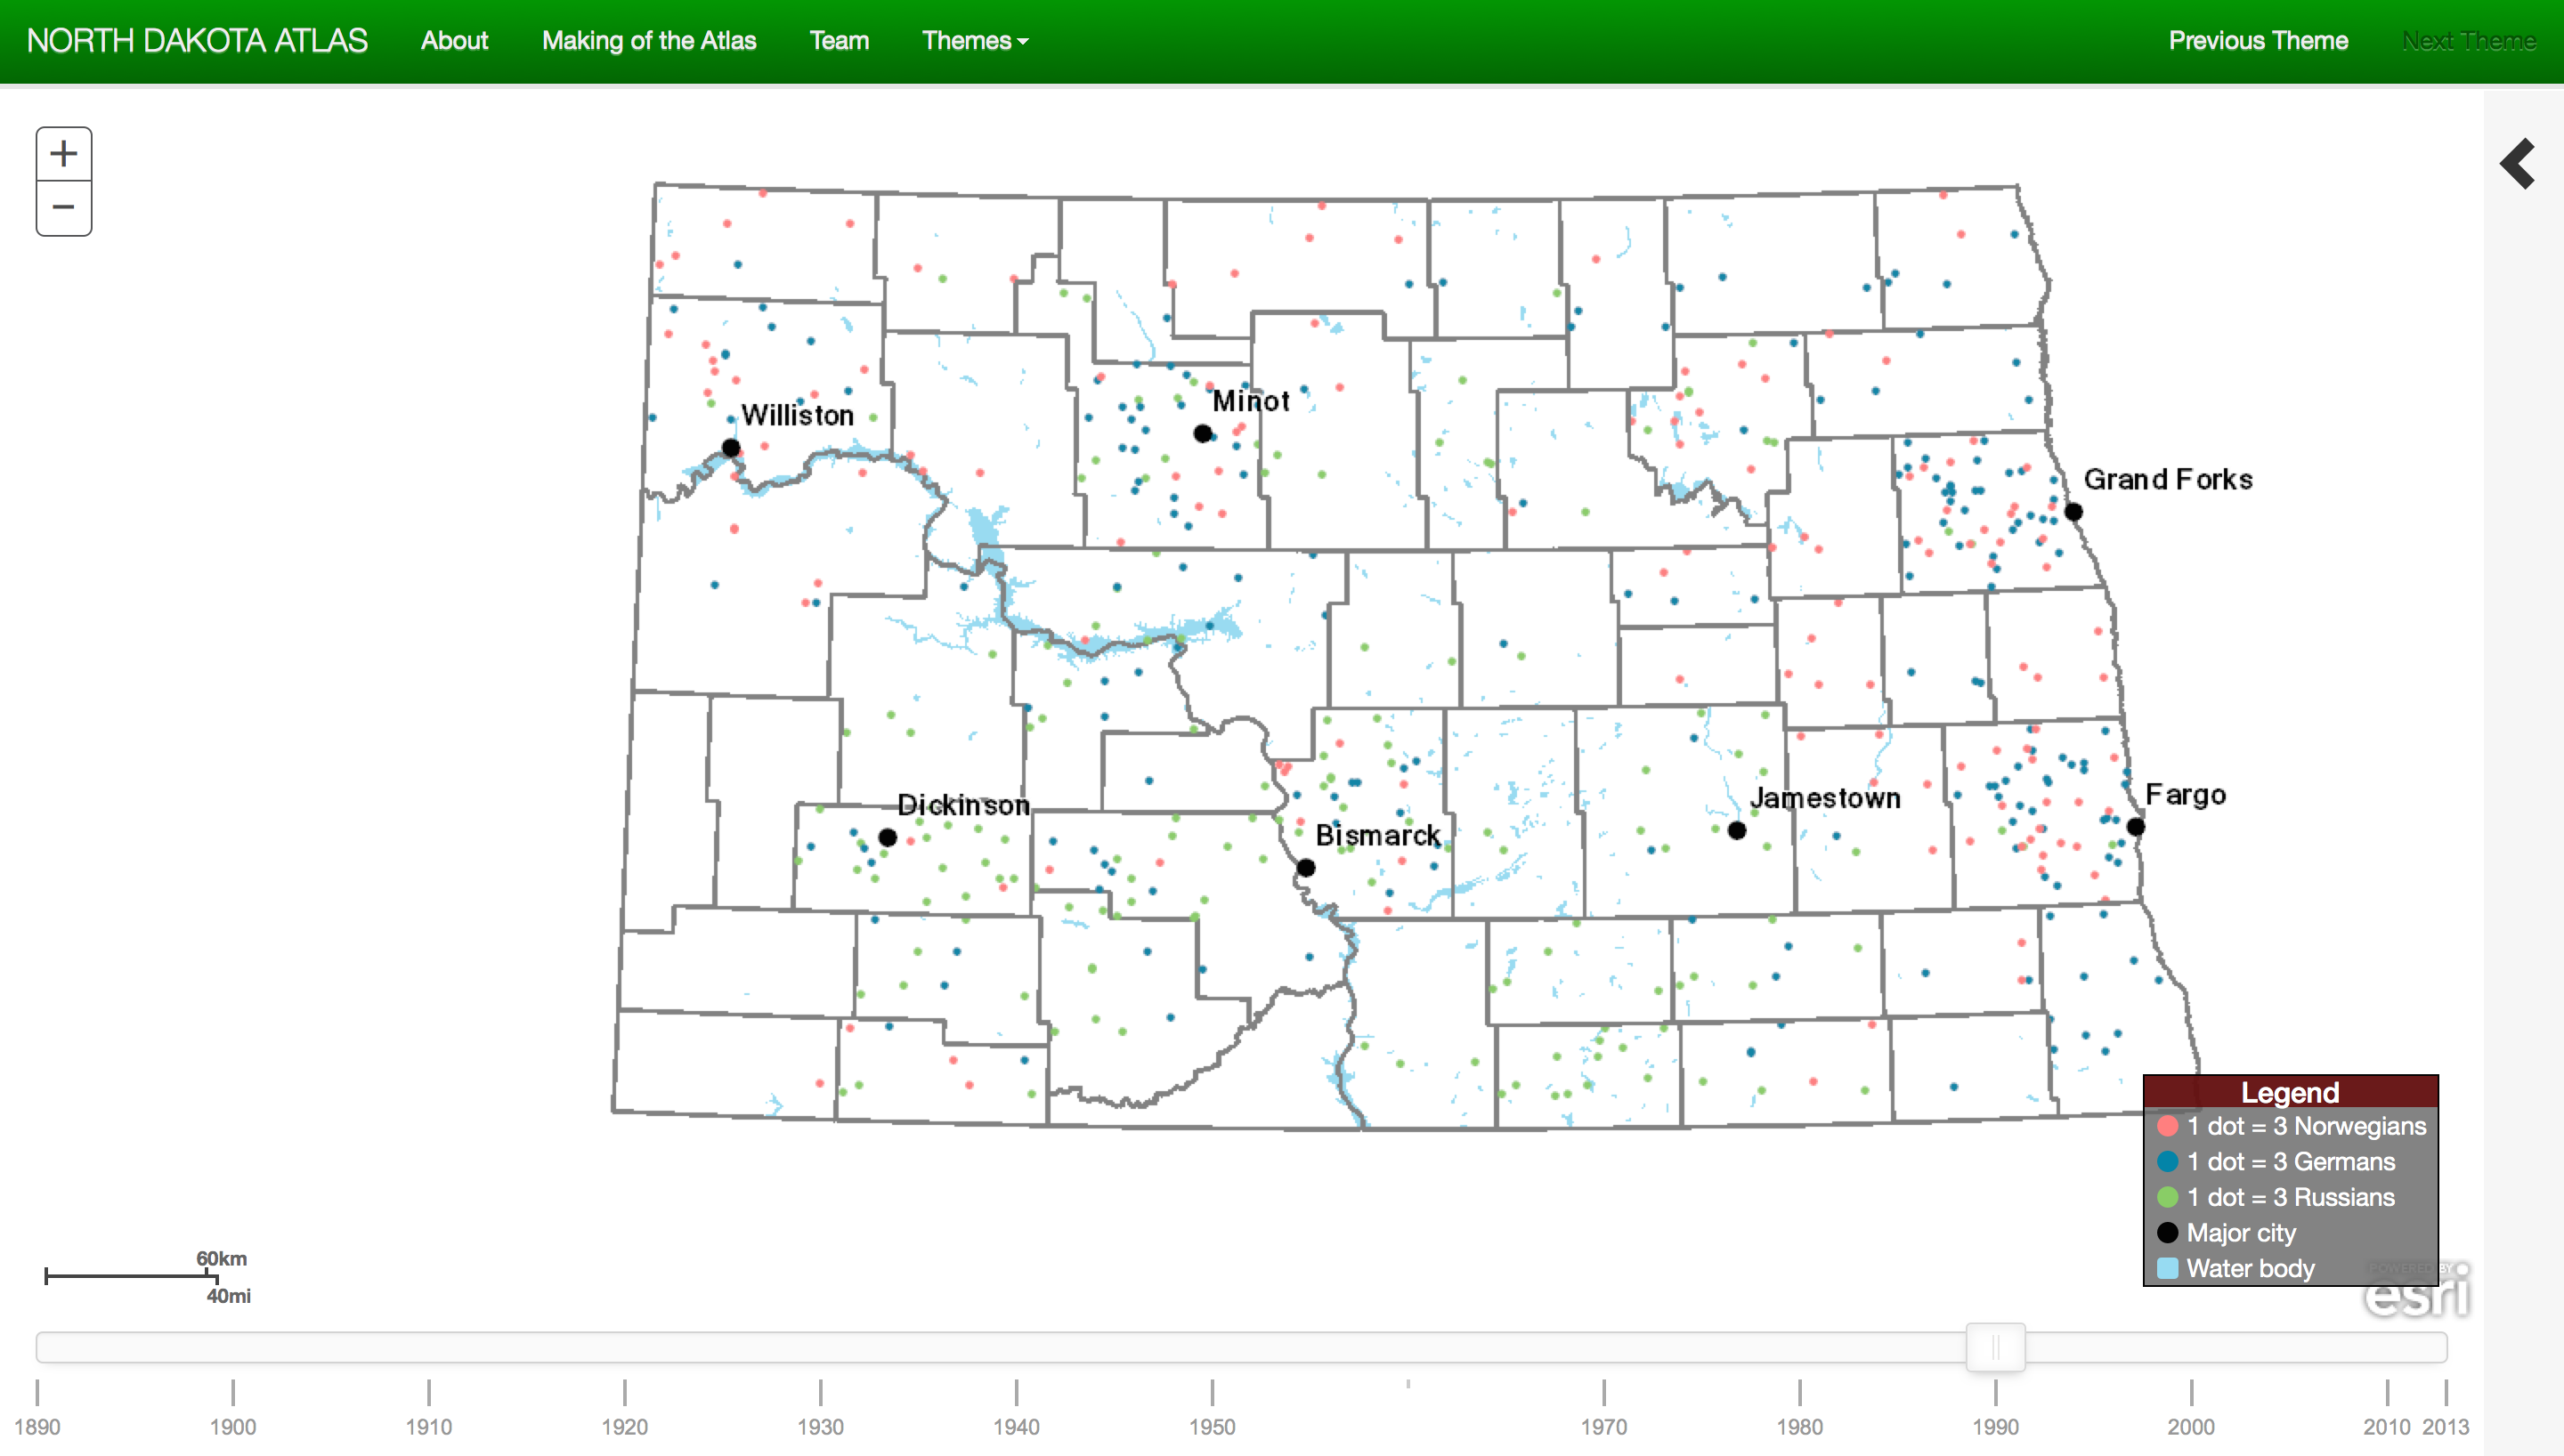
\includegraphics[width=0.45\textwidth]{ancestry_no_narrative}
	\caption{Example of map with a hidden narrative.}
	\label{fig:ancestry_no_narrative}
\end{figure}

\subsection{Navigation Bar}
The navigation bar is an extremely important element in AtlasCMS. Visible on every page, and remaining at the top of the page even as the user scrolls, the navigation bar must be automatically adjusted based on the page being viewed. Figure~\ref{fig:home_themes} shows the navigation bar, with the Themes clicked, on the landing page. This shows a drop down with both themes, allowing the user to quickly navigate to an individual theme. Additionally, the user can click NORTH DAKOTA ATLAS to return to the landing page, or About, Making Of, or Team to navigate to the corresponding section on the landing page.

\begin{figure}[h!]
	\centering
	
\includegraphics[width=0.45\textwidth]{home_themes}
	\caption{Navigation bar on the landing page.}
	\label{fig:home_themes}
\end{figure}

The navigation bar automatically adjusts depending on the theme being viewed. As shown in Figure~\ref{fig:making_themes}, with Themes clicked, the list of both themes are shown, just like on the landing page. However, since we are on the History of the State theme, it is presented in bold font, indicating that it is the current view. This allows the user to confirm the theme they are on quickly, while selecting a new theme. Additionally, a Next / Previous Theme button is provided at the right of the navigation bar (not shown), allowing the user to easily navigate to the corresponding theme, if available.

\begin{figure}[h!]
	\centering
	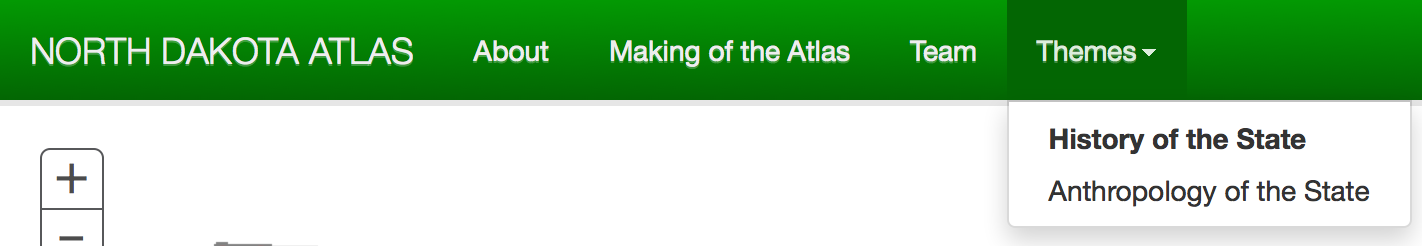
\includegraphics[width=0.45\textwidth]{making_themes}
	\caption{Navigation bar on the History of the State theme.}
	\label{fig:making_themes}
\end{figure}

\section{Future Work}
There are three main focuses that are suggested for future work, in order of importance: the completion of the CMS portion of AtlasCMS; the full scalability to multiple viewports; and ability to use GeoJSON and OpenMaps (or alternative open-source mapping technology), to remove the need for ArcGIS Server.

The CMS portion of AtlasCMS is only partially functional, allowing the creation of themes, deletion of themes, and adding of stories and sections to themes. However, all of this is done in blocky text areas. To aid in usability, the CMS portion should us a WYSIWYG editor, similar to Microsoft Word, to allow non-technical persons to quickly and easily update content.

AtlasCMS has the ability to scale to multiple viewports thanks to the Bootstrap framework, and the navigation bar and landing page have been built with this scalability in mind. However, the map pages are not currently well suited to smaller viewports, with the narrative taking up a significant amount of screen real estate. The map view will need to be modified, based on viewport, to not show the narrative on smaller viewports by default, and having the narrative fill the entire screen when show. Additionally, touch features, such as swiping in the narrative, should be included for more portability to different devices. 

AtlasCMS is custom made for a situation in which an ArcGIS Server is available. Creating an interface that uses fully open standards such as GeoJSON and OpenMaps, while allowing the same level of interaction currently provided by ArcGIS Server would be ideal. This would allow AtlasCMS to be used be a wider variety of projects at zero cost. However, to incorporate this functionality, a specific set of expected variables in the GeoJSON must be defined by the program and created by the content managers, removing some of the ease-of-use of AtlasCMS.

\section{Conclusion}
The AtlasCMS project successfully showcases that an interactive online atlas that works across multiple viewports, displaying maps related to the 125 year anniversary of North Dakota is possible. This not only allows students, teachers, and people interested in history to interact with various aspects of North Dakota history, but is easily extendible to other projects. The biggest obstacle for AtlasCMS is fulfilling the CMS portion of its name in a user-friendly manner.

Given the open source nature of the project, North Dakota related branding should be removed from the project, with future development focusing on creating a robust CMS to make use of the front-end features displayed during this project. Users will then be able to install AtlasCMS as a Node.js project in 2 lines and start creating their own online atlas - hopefully with the ability to use other open frameworks, such as GeoJSON and OpenMaps in the near future. The potential to convert physical atlases quickly and easily into an interactive form, with minimal need for a developer, has significant potential in the academic field to digitize content so that more people can benefit from it.

\bibliographystyle{IEEEtran.bst}
\bibliography{references.bib}

\end{document}
